\documentclass[a5paper, 11pt, openany]{book}
\usepackage{ctex}

\usepackage{geometry}
\geometry{left=1.8cm,right=1.8cm,top=2cm,bottom=2cm}
\usepackage{hyperref}
\usepackage{graphicx}
\usepackage[export]{adjustbox}
\usepackage{amsmath}
\usepackage{subfigure}
\usepackage[utf8]{inputenc}
\usepackage{microtype}
\usepackage{pythonhighlight}
\frenchspacing

\graphicspath{ {./figures/} }
\title{\textbf{\huge AI技术入门:神经网络基础 \\ \Large MLP ABC}}
\author{李孙博闻\thanks{E-mail: bw1863@outlook.com}}
\date{\today}

\begin{document}

\maketitle
\newpage

%%%%%%%%%%%%%%%%%%%%%%%%%%%%%%%%%%%%%%%

作者简介:一个学习机器学习的的普通人\\ \\

github主页 \href{https://github.com/Aegis1863} {https://github.com/Aegis1863} \\ \\

下载最新版文档请移步更新发布页:

\href{https://github.com/Aegis1863/MLP-ABC/releases/}{https://github.com/Aegis1863/MLP-ABC/releases/} \\ \\

欢迎提交issue或pull request。
%%%%%%%%%%%%%%%%%%%%%%%%%%%%%%%%%%%%%%%

\chapter{前言}
关于神经网络的教学多如牛毛,在任何涉及机器学习的书中,几乎都会介绍神经网络基础,撰写此小册子也不过多此一举,但在大量实践之后,产生了不少新的理解,还有一些是在初学时就理解错的,\textbf{因此撰写此书,总结对神经网络的认识,也是对教会我机器学习基础的书\footnote{《机器学习实战-基于Scikit-Learn、Keras和Tensorflow》,第二章有介绍。}的作者Aurélien Géron的致敬}。神经网络原理只是深度学习的基础知识,但真正写本书时,发现其细节之多也难以介绍完全,本书的目的就在于阐释笔者对于神经网络的全部理解,有些部分对初学者来说可能比较超前,可以学到后面再回头看看,但仍不涉及太深奥的数学推导,读者具备大学数学基础即可阅读。

学习本书,需要具备一定的高数知识,例如链式求导法则,\textbf{需要熟悉概率论},需要具备一定的线性代数知识,例如在计算方面涉及到矩阵的简单运算,并且建议自行在网络上查找观看神经网络运作机制的视频,有一个大致了解后看本书更有帮助,同时鼓励读者通过其他资料补充学习。

新手通常在学习基本编程的同时学习机器学习,在这种情况下一旦碰到报错,通常只能求助于人或者网络,这又需要很强的信息检索能力,新手提问还需注意提问方法,告知程序环境、报错信息等,也先用截图的方式(切忌手机拍照)告知关键报错是什么,再进行补充,否则可能无人应答,这种情况下也不要气馁,无人应答可能是因为别人不是此领域、没时间或没看懂报错等,这并不尴尬;当然,如果你的问题恰好是别人已经碰到并且解决过的,那么ta大概率会回答你的问题,但不要指望太多:\textbf{无人应答才是常态},学习者应该尽量尝试自己解决问题。

学习基础和巩固代码能力是很重要的,因为这是培养自己独立理解报错和排查错误能力的关键途径——须知,在学习过程中碰到的报错只会越来越多而不会越来越少。幸运的是Python和大部分常用包的报错反馈是比较清晰的。

笔者建议认真阅读第\ref{单个感知机}章单个感知机及其后面的所有部分的内容,有的地方刚开始不懂,可以跳过,看到后面之后可以再对照翻回来看看。第\ref{神经网络章节}章会展示如何用现成框架搭建神经网络,也会展示如何自行编写一个简单神经网络,其代码基于笔者完成的一个简单BP神经网络实例\href{https://github.com/Aegis1863/ML_practice/blob/master/机器学习笔记/X_01_手搓BP神经网络.ipynb}{<手搓BP神经网络>},链接\label{代码链接}如下:
\begin{verbatim}
https://github.com/Aegis1863/ML_practice/blob/master/
机器学习笔记/X_01_手搓BP神经网络.ipynb
\end{verbatim}


由于笔者能力有限,难免有错误和疏漏,欢迎联系笔者并且指正。

\section{提示}
\begin{center}
    < > : 如果你看的是电子版,小书名号通常是可以打开的链接 \\
    \textbf{黑体加粗部分表示强调}
\end{center}

%%%%%%%%%%%%%%%%%%%%%%%%%%%%%%%%%%%%%%%

\tableofcontents

%%%%%%%%%%%%%%%%%%%%%%%%%%%%%%%%%%%%%%%
\chapter{他山之石}
笔者在这方面的学习历程也并不算顺利:其中学习基本的Python编程学习了大约1个月,本科4年期间主要沿着数据科学的路线学习,通过自己训练或者参加比赛的方式锻炼基本编程能力和处理报错的能力,本科毕业之后以较多的精力在5个月左右完成机器学习基础的学习(跨度两年),也就是笔者撰写本文的这个时期。

这里简单介绍笔者的学习经历,也是机器学习领域比较认可的路径之一\label{route}:
\begin{enumerate}
    \item 传统机器学习\footnote{传统机器学习不是本文的重点,同时如果重心放在深度学习,也的确不用花太多精力理解传统机器学习原理,会使用现成的包例如Sklearn即可,不作具体说明}
        \begin{enumerate}
            \item 线性模型:\textbf{从这里开始,读者应该从统计学思想过渡到机器学习思想,这意味着对模型的评价方法有很大变化,例如不再过多关注统计量是否显著,实际上,对于一个机器学习学习者来说,从此不再有统计量这个概念}。
            \item 支持向量机
            \item 决策树/随机森林
            \item XGBoost
        \end{enumerate}
    \item 深度学习
        \begin{enumerate}
            \item 多层感知机(MLP):所有神经网络的基础,本文重点
            \item 卷积神经网络(CNN):图像处理的基础技术
            \item 循环神经网络(RNN):时间序列的基础技术
            \item 编码器:AI歌手和图像生成等技术的基础技术
            \item 生成对抗神经网络(GAN):AI绘画等的基础技术
        \end{enumerate}
    \item 强化学习:笔者撰写本文时的主要研究内容,需要有深度学习的基础,特点是结构复杂,难度大,消耗资源多,现成可用的包少。
\end{enumerate}

\section{书籍和视频资料}
这里的推荐分两个部分,一个是笔者自己系统学习过的资料,另一个是网上比较推荐的资料,只是提供一个来源,并非商业推广,从什么渠道看或者购买,读者可自行决定:

\begin{enumerate}
    \item 自学材料
    \begin{enumerate}
        \item \href{https://www.bilibili.com/video/BV1JF411L7SD}{<视频>Python基础},北京理工大学嵩天的系列视频课程都很推荐,笔者从该系列课程中学习了基础编程、数据科学、可视化方法和简单爬虫技术。\label{视频课程}
        \item \href{https://detail.tmall.com/item.htm?abbucket=0&id=629528559505D}{<书>机器学习实战(第二版)}此书对新人很友好(要熟练基础编程),对数学原理的解释点到为止,重点在于引导读者写出代码,提供了详细的代码示例和大部分人可以接受的学习曲线,包含<\ref{route}>中的全部内容,笔者也只是从这本书中学到一些皮毛,但也受益匪浅。
    \end{enumerate}
    \item 其他推荐,难度比较高,建议中后期学习
    \begin{enumerate}
        \item \href{https://detail.tmall.com/item.htm?ali_refid=a3_430582_1006:1106222247:N:H6LEKWw5w+wEVaha6Pu0Aw==:5d2ca6404d6e3a2c4c17a9259c4bff4f&ali_trackid=1_5d2ca6404d6e3a2c4c17a9259c4bff4f&id=540848628472}{<书>机器学习},也叫西瓜书,国内最好的教材之一,但正如前面所说,有一定难度,没有详细代码。
        \item \href{https://detail.tmall.com/item.htm?abbucket=0&id=638756997988&ns=1&spm=a21n57.1.0.0.f353523cYBsNmp}{<书>机器学习公式详解},也叫南瓜书,是上一本西瓜书的公式推导手册。
        \item \href{https://detail.tmall.com/item.htm?abbucket=0&id=555191140768&ns=1&spm=a21n57.1.0.0.5ae1523cue95nE}{<书>深度学习},也叫花书,大佬称为圣经,但笔者在中后期才能勉强看懂QAQ。
        \item \href{https://www.bilibili.com/video/BV1H44y1t75x}{<视频>李沐论文精读系列视频},李沐大神的带读论文视频,价值极高。
    \end{enumerate}
    \item 一些机器学习专家建议把整个数学体系都学习过之后再学机器学习,此路径很消耗时间,也很困难,除非天赋异禀。当然,数学能力实际上决定了在这个专业方向的天花板,尽管本书中只强调了高数、概率论、线性代数,但希望读者能在学习过程中尽量提高自己的数学水平,能够推导的部分尽量手推。
\end{enumerate}

\begin{figure}[ht]
    \centering
    \subfigure[机器学习]{
    
\includegraphics[width=0.3\textwidth]{figures/西瓜书.png}}
    \subfigure[机器学习实战]{
    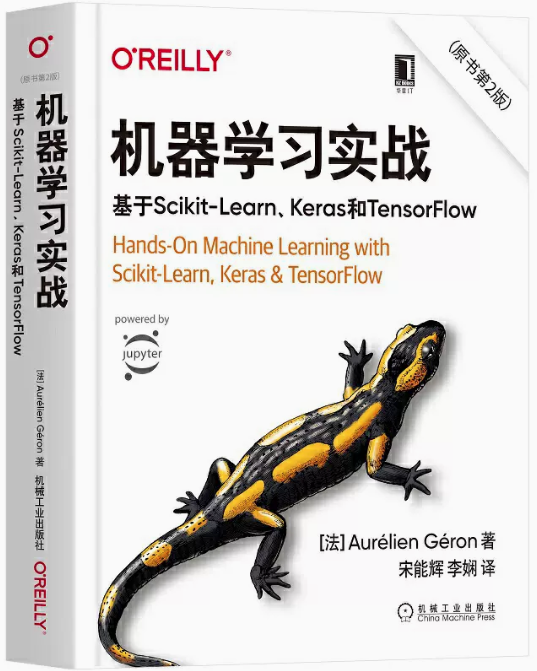
\includegraphics[width=0.3\textwidth]{figures/机器学习实战.png}}
    \subfigure[深度学习(花书)]{
    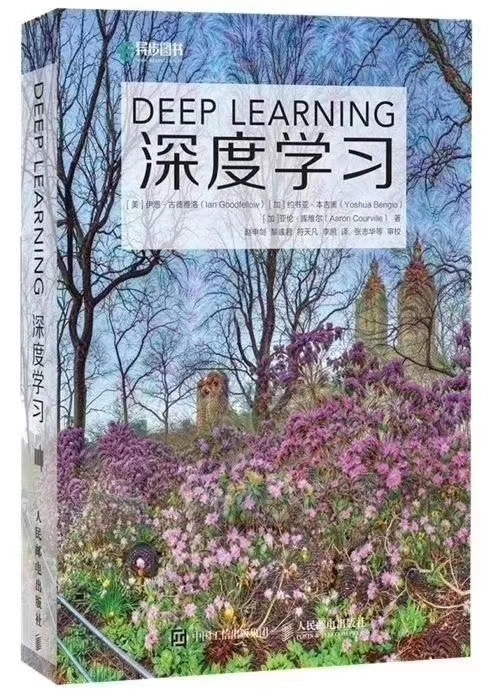
\includegraphics[width=0.3\textwidth]{figures/花书.png}}
    \caption{部分推荐书籍}
\end{figure}

%%%%%%%%%%%%%%%%%%%%%%%%%%%%%%%%%%%%%%%
\chapter{单个感知机} \label{单个感知机}

\section{单个神经元的结构}
感知机也就是神经元,是MLP\footnote{多层感知机: Multi-Layer Perceptron}的基本单元,这里先学习单个感知机是如何传递信号的。我们在神经网络图像中一般用一个圆来表示一个感知机,一个感知机自带两个公式,一个是$y=wx+b$,$w$也叫权重,$b$也叫偏置项,我相信这不难理解,另一个是激活函数,\label{为什么用sigmoid}与生物神经元性质最接近的激活函数是$sigmoid$,如图\ref{sig}和公式\ref{公式1}。而单个感知机的结构如图\ref{neuron structure},我相信它的信息是不言而喻的:x进入感知机后经过两步运算得到一个输出,这个输入传递给下一层所有的神经元,而每个神经元几乎都是一样的,这没有什么新鲜的,对吧!

注意:此时$y$和$x$是已知的,就像我们事先知道了100个x与y的值,要求的是$w$和$b$,在这以后,给定任意的$x$就可以得到一个$y$。$w$和$b$在一开始会被随机赋值,比如从正态分布中抽两个随机数给它们,在后续计算中,它们的值会一直被修改,在修改若干次后停止,最终的值就是我们的估计,换句话说,它们是\textbf{需要被估计的参数},而$sigmoid$函数里面没有未知数,也就是说激活函数只是改变这个神经元最终输出的形状,没有未知参数。

\begin{figure}[ht]
    \centering
    \subfigure[sigmoid函数]{
    \label{sig}
    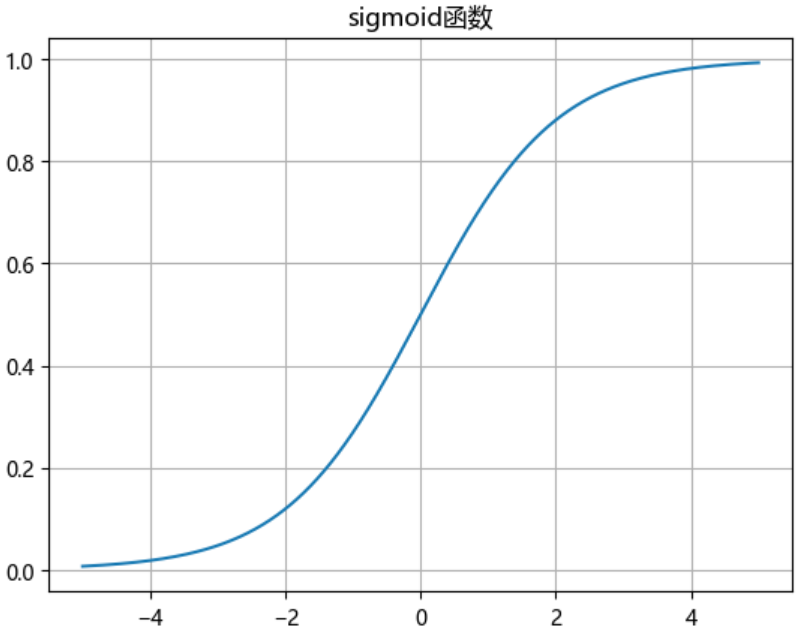
\includegraphics[width=0.6\textwidth]{figures/sigmoid.jpg}}
    \subfigure[神经元结构]{
    \label{neuron structure}
    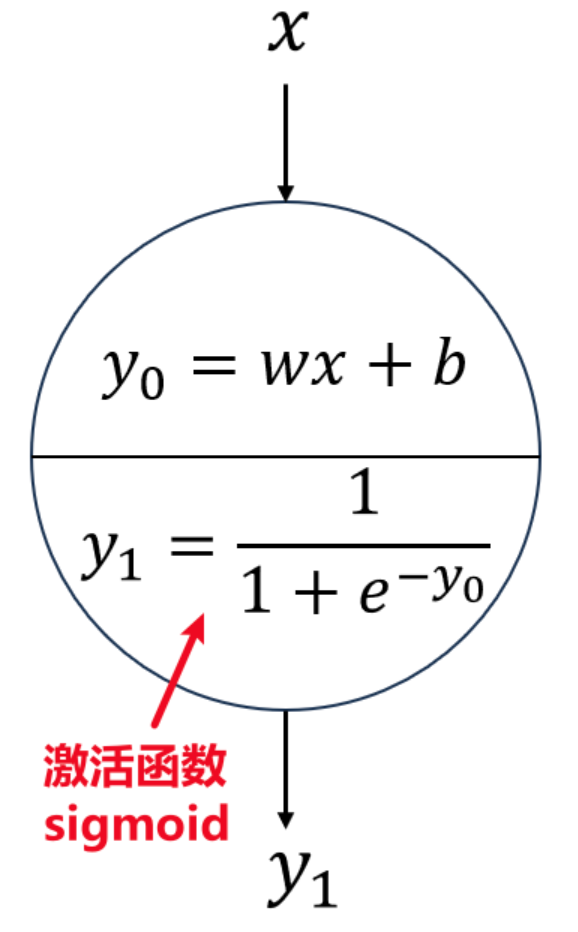
\includegraphics[width=0.29\textwidth]{figures/神经元.png}}
    \caption{激活函数和神经元结构}
    \label{figure1}
\end{figure}

\begin{equation}
    \begin{cases}\label{公式1}
        y=wx+b \\
        sigmoid(x) = \frac{1}{1+e^{-x}}
    \end{cases}
\end{equation}

在上述条件下,一个神经元的真正输出公式就是把$y=wx+b$带入$sigmoid$:
\begin{equation}\label{sig_y}
    y = \frac{1}{1+e^{-wx+b}}
\end{equation}

如果此时我要求你对式子\ref{sig_y}计算$\frac{dy}{dx}$,那么你(大概)很快就能写出式子。实际上$sigmoid$函数很适合做求导,我们把它简单写成$\sigma(x)$:

\begin{equation}
    \sigma'(x) = \frac{e^{-x}}{(1+e^{-x})^2}=\sigma(x)(1 - \sigma(x))
\end{equation}

如果考虑式子\ref{sig_y},就仅仅需要把$w$乘到里面,$w$是矩阵,求导之后需要转置,也就是$\sigma(x)(1 - \sigma(x))w^T$,是不是真的很简单,对一个函数求导只需要调用它自己的函数两次,这里就已经有迭代的思想了,在整个机器学习框架中都或多或少有这种思想,强化学习更甚,即下一个状态可以由上一个状态的值计算而来,这非常适合用来编程,因为函数是可以重复利用的,它不需要太多其他的运算。

\section{激活函数}
$sigmoid$是一个S形函数,并且在x取无穷大或者无穷小时,其导数接近0,因此也叫饱和激活函数,类似的还有$tanh$,激活函数有很多种,\textbf{神经网络拟合函数是靠多个线条组合成的},一个线条来源于一个感知机,这个线条可以是直线,也可以是曲线,它的形状取决于激活函数,激活函数是$sigmoid$时,单个线条就是一个曲线,当然,如果把曲线分割成无数段,它也可以是直线的形状。

\begin{figure}[ht]
    \centering
    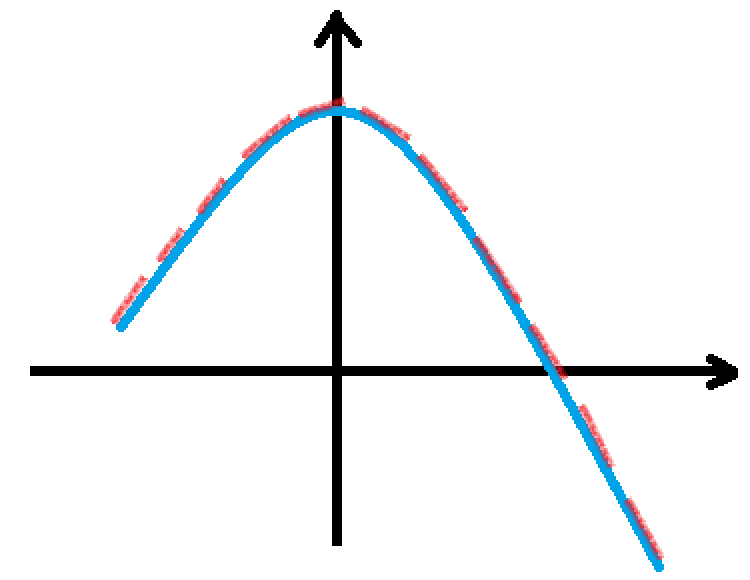
\includegraphics[width=0.4\textwidth]{figures/拟合线.png}
    \caption{多个神经元组成的线段拟合原始曲线}
    \label{手画拟合线}
\end{figure}

正如本节刚开始说的<\ref{为什么用sigmoid}>,人们早期使用$sigmoid$只是因为它类似真实生物的信号传递特征,但它并不是最优的,它的求导看起来确实非常简单,但能不能更简单呢,最简单的求导是一元一次方程,$x$的导数就是它的系数,并且,激活函数换成直线好像也并不冲突!被无限分割的直线还是直线,被无限分割的曲线呢?每一个部分也是“直线”!

于是现代最常用的激活函数$ReLU$呼之欲出:

\begin{equation}
    \label{Relu函数}
    ReLU(x) =
    \begin{cases}
        0 & \text{if } x \le 0,\\
        x & \text{if } x > 0.
    \end{cases}
\end{equation}

当$y=wx+b$的结果小于0的时候,经过激活函数后输出为0,也就是说它此时"死亡",但不代表与它连接的下一个神经元也“死亡”,因为一个神经元实际上要接受上一层所有神经元的信号并且加起来,参考图\ref{figure2},每个神经元初始的$w$和$b$是不一样的,不可能前面那层全都是0吧!这有助于防止过拟合,试想,本来5个线段就可以拟合好的函数,现在放置了20个神经元,那么至多有15个神经元是不必要的,它们凭空增加了计算复杂度,但是残差连接可以改善此问题,在\ref{残差连接}中具体讨论。ReLU可以关闭接近一半的神经元:考虑到$w$和$b$刚开始是被认为初始化的,它们被赋予某种分布的某个随机值,通常是标准正态分布的,因此经过公式\ref{公式1}一式输出的$y$也是正态分布的,$y$小于0的那些神经元就被关闭。

在输出层,如果是回归任务,则没有激活函数,如果是二分类任务,采用$sigmoid$激活函数,如果是多分类任务,采用$Softmax$函数。

%%%%%%%%%%%%%%%%%%%%%%%%%%%%%%%%%%%%%%%

\chapter{神经网络} \label{神经网络章节}

\section{不同激活函数的表现}

\begin{figure}[ht]
    \centering
    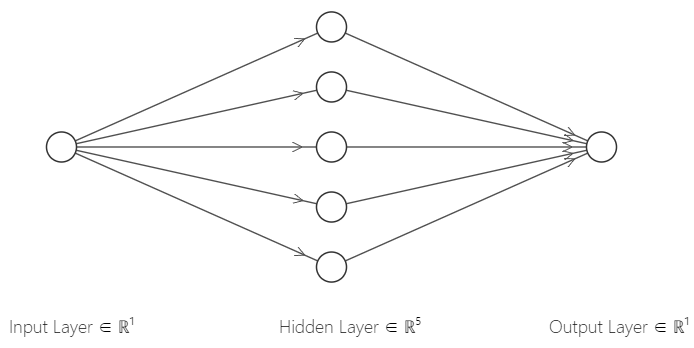
\includegraphics[width=0.9\textwidth]{figures/神经网络.png}
    \caption{多个神经元组成的神经网络}
    \label{figure2}
\end{figure}

现在我会展示一下激活函数的不同会导致什么样的拟合现象,我创建了一些散点,它们大致表现为函数$y=2sinx$,我相信这个函数的图像对你而言非常清晰,我在每个点的$y$值上随机地进行了标准正态分布的随机数加减以打散它们。

在图\ref{figure3}我画了一条红色的线,那是通过统计学的最小二乘法公式得来的(赞美数学),如公式\ref{最小二乘法},你可能会觉得很复杂,这还是一元一次的情况,在更高维度下,求解公式会越来越复杂,幸好,我们的神经网络就是解决这个问题的,它提供了一个替代方法逼近原函数。

\begin{equation}
    \begin{cases}
        w = \frac{n\sum{xy}-\sum{x}\sum{y}}{n\sum{x}^2-(\sum{x})^2} \\
        b = \overline{y} - w * \overline{x}
    \end{cases}
    \label{最小二乘法}
\end{equation}

\begin{figure}[ht]
    \centering
    \subfigure[sigmoid激活]{
    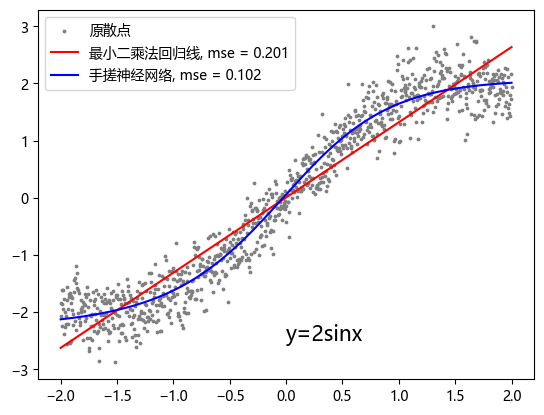
\includegraphics[width=0.48\textwidth]{figures/sigmoid激活.png}}
    \subfigure[ReLU激活]{
    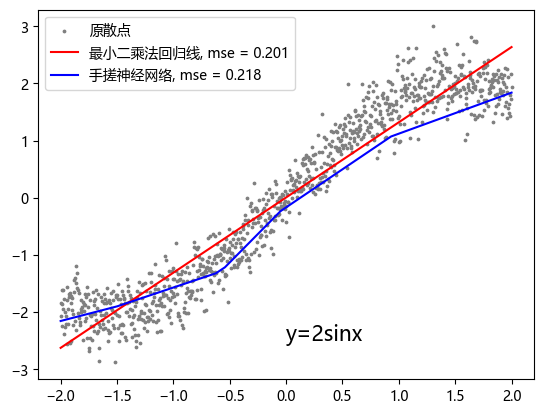
\includegraphics[width=0.48\textwidth]{figures/relu激活.png}}
    \caption{不同激活函数拟合的样子}
    \label{figure3}
\end{figure}

同时我手搓了一个隐藏层有五个神经元的神经网络,我建议你也定一个目标,即未来某一天写出自己的神经网络,这可是你吃饭的家伙!这个手搓网络的结构正如图\ref{figure2},它有一个输入层,一个隐藏层,一个输出层,其中输入层是没有参数的,就是$x$。当激活函数是$sigmoid$的时候,它表现得很好,如图\ref{figure3},因为图像本身就是s型,用s型的激活函数自然表现最好,但我用ReLU时,它用几段折线的组合去拟合散点,理论上应该有5根折线,对应5个神经元,也表现得不错(吗),但是如果我使用更多神经元,如100个神经元,我们会有100个小线段,这种拟合当然会更好,你可以看看前面的图\ref{手画拟合线}。此外,增加层数也可以有很大的提升,增加一层神经元就可以加一维的分类或拟合的能力,以此类推,试想两个面包片上下夹在一起,垂直划分是不可能分开的,但是水平切一刀就可以分开,这就是增加神经网络层数的作用。

神经网络也可以更复杂,如图\ref{figure4},它有一个输入层,包含2个神经元,对应2个特征,两个隐藏层,各有4个和6个神经元,一个输出层,包含1个神经元,表示输出1个值,输入层没有参数,所以一般不认为是单独的一层,而隐藏层和输出层有参数,每一个神经元的$w$的数量等于上一层神经元数量,但是一个神经元只有一个$b$。

我们可以做一个简单的计算:上一层有4个神经元,下一层有6个神经元,那么下一层就有$4*6+6=30$个需要估计的参数,其中4是上一层神经元个数,6是下一层神经元个数,因此下一层有24个$w$,加6是因为下一层每个神经元各有一个$b$,也叫偏置项。

\begin{figure}[ht]
    \centering
    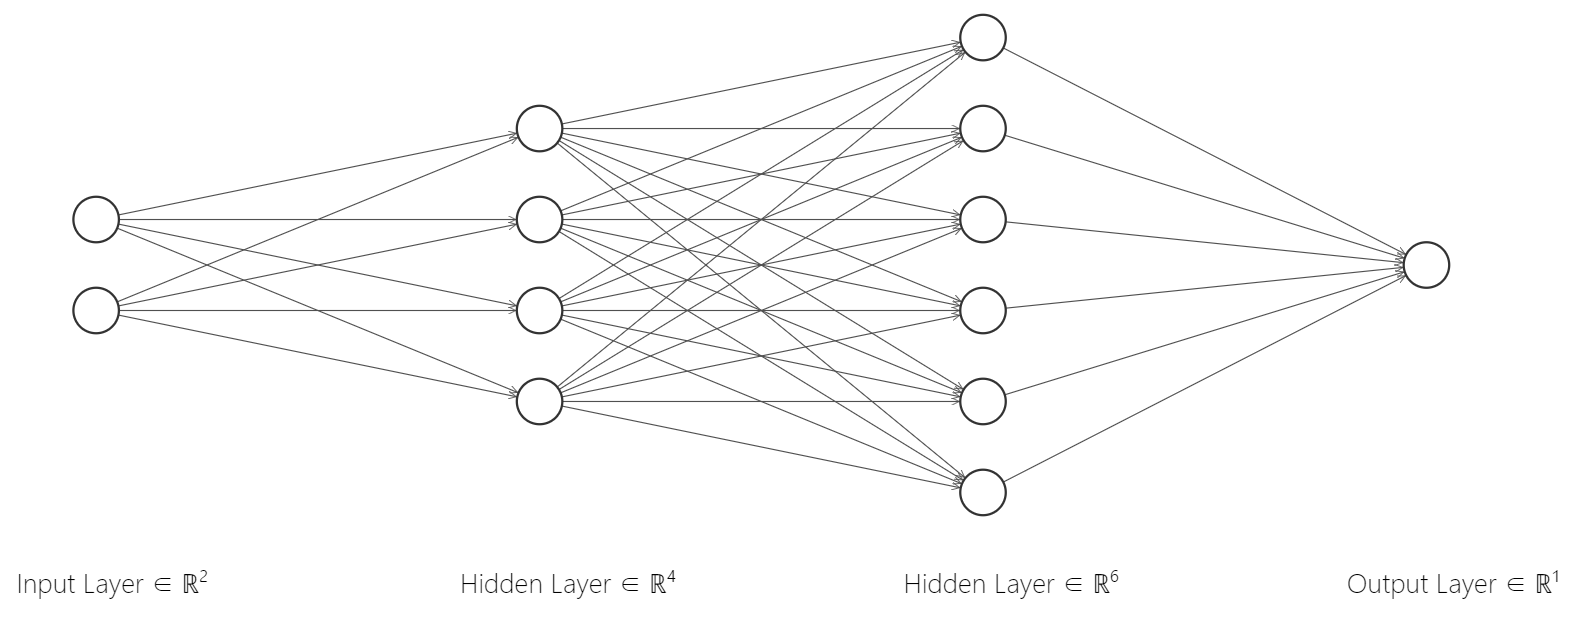
\includegraphics[width=\textwidth]{figures/复杂神经网络.png}
    \caption{比较复杂的神经网络}
    \label{figure4}
\end{figure}

\section{正向传播}

观察图\ref{figure4},数据从神经网络的左边进入,通过神经元计算传递到下一层神经元,最后从最右边的神经元输出一个值或矩阵,在机器学习领域,这些在神经网络中流动的矩阵,我们通常称为张量\footnote{大多数人习惯把二维数组称为矩阵,高维数组称为张量,但是有时候可以混用,如一维张量,也就是向量;二维张量,也就是矩阵;三维张量等。}。这些神经元是全连接的,即每一个神经元都要与下一层所有神经元连接起来,因此也可以称之为全连接神经网络,其含义与MLP基本一样。这里我们有两个隐藏层,它具有划分三维数据的能力,用来处理二维数据更是绰绰有余。

\begin{table}[ht]
    \centering
    \begin{tabular}{c c c c}
      index & 模拟考试A & 模拟考试B & 期末考试  \\ \hline
         1  & 85     &   76     &  80      \\ 
         2  & 76     &   83     &  80      \\ 
         3  & 90     &   86     &  87      \\
         4  & 70     &   80     &  73      \\
         ...&  ...   &   ...    &  ...
    \end{tabular}
    \caption{成绩单}
    \label{table1}
\end{table}

机器学习所需的数据,形式上类似常见的那些表格,我们规定一列为一个特征,或者称字段\footnote{虽然特征和字段所指代的东西基本相同,但不同场合仍然有不同叫法。},假如我们现在有一份数据,它有三个字段,前两个是模拟考试A和B的分数,第三个是期末考试的分数,如表\ref{table1},实际上在深度学习任务中,你大部分时候都要准备这样的表格,例如xlsx或者csv格式的表格,它必须包含若干特征列,并且包含一个目标列,通常是最后一列,例如这里的期末考试成绩,你必须有若干条这样的已知数据,例如100条甚至10000条,才能用于训练网络,因为网络是通过迭代来训练参数的,如果数据太少,迭代就难以进行,泛化能力也就不理想,通常我会用70\%的数据训练,15\%的数据用于验证,15\%的数据用于测试,这些数据不能混淆,在一开始就应该做出区分,否则称为数据集污染。

假如此时模型的任务是通过两次模拟考试的分数推断期末考试的分数,我们需要训练模型,单个输入的大小就是[2, 1],也就是两行一列的二维张量,想象一下把表格的特征列转置过来,然后推进神经网络的左边,由于神经网络中每个神经元的参数$w$和$b$都在被建立时随机赋值了,因此模型可以在最右边输出一个数字,然而这个数字大概毫无意义,它可能是200,可能是-30,然而真实的是80,显然,如果我们改变$w$和$b$的取值,就能改变模型最终输出的值,因此我们可以让$w$和$b$的值改变,从而使模型的输出趋近于80,这个过程就是训练,具体来说是通过梯度下降法来进行训练。从这里可以看出来,机器学习也只能学习到确有关联的数据特征,如果要拟合体重和成绩,结果通常不好并且没有意义。

要注意的是,有时候虽然我们有很多数据,但它们不一定真的存在某种有意义的关系,训练的结果可能很差,甚至有时候神经网络的确得到了一个不错的效果,但是变量间实际上毫无逻辑关系,就像统计学中的伪回归一样。\textbf{再次强调,一个拥有足够多神经元和足够多层数的神经网络在理论上的确可以拟合所有函数,但它绝不是什么灵丹妙药,因为我们难以解释神经元的行为逻辑,统计学模型可解释性更强。}

\begin{figure}[ht]
    \centering
    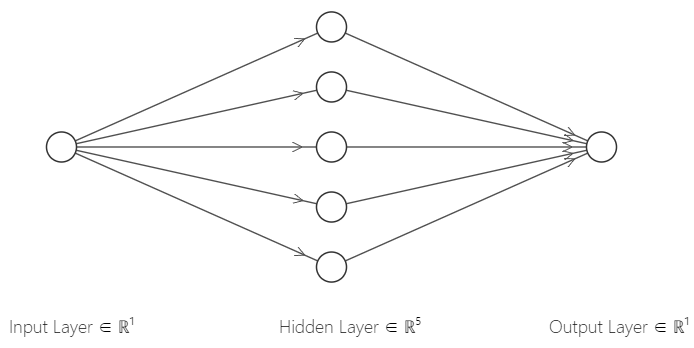
\includegraphics[width=0.8\textwidth]{figures/神经网络.png}
\end{figure}

我们以图\ref{figure2}的网络为例,最左边的输入层是$x$,由于输入层没有参数,通常也不认为是单独的一层,中间的是一个包含五个神经元的隐藏层,最后是一个神经元构成的输出层,向前传播公式表示为式\ref{forward}。

\begin{equation}\label{forward}
    \begin{aligned}
        hidden\_layer: 
        \begin{cases}
            y_{11} = w_1x+b_1 \\
            y_{12} = \frac{1}{1+e^{-y_{11}}}
        \end{cases}\\
        output\_layer:
            y_{21} = w_2y_{12} + b_2
    \end{aligned}
\end{equation}

这里的$w, x, b$都是以矩阵形式进行运算的,$w_1$表示隐藏层权重,$b_1$表示隐藏层偏置项,以此类推,$y_{11}$表示隐藏层第一次运算结果,$y_{12}$表示隐藏层第二次运算结果(激活函数),$y_{21}$表示输出层第一次运算结果,没有激活函数。

\section{梯度下降和反向传播}

你应该知道正向传播是如何进行的了(吧),在一次正向传播之后会伴随一次反向传播,即通过梯度下降的方法修正$w, b$,它们一开始是被随机赋值的,我们希望修正它们从而使得模型输出的数字越来越接近已知的真实数据。

我们必须先定义一个损失函数$loss$,比如真实值$y_{true}$是80,模型预测出$y_{21}$为84,那么此时误差不是很大,若模型预测出1000,那么误差就显然很大,但是模型是程序,只认数字,因此我们必须给出一个式子来衡量这种差异。统计学中已经给出了方案,就是方差,如公式\ref{loss函数},也被称为均方差,英文简写MSE(Mean Square Error),不同的是这里的系数是$\frac{1}{2}$,而在统计学中,应该是$\frac{1}{n}$或者$\frac{1}{n-1}$,这样处理是为了方便求导,在求导的时候,平方项和$\frac{1}{2}$会直接抵消,而这个系数只是对损失有缩放,因此没有什么影响。你可能注意到了,这是第二次提到“方便求导”。

\begin{equation}\label{loss函数}
    loss(y_{21}, y_{true}) = \frac{1}{2}\sum(y_{21} - y_{true})^2
\end{equation}

现在我们有一个衡量损失的函数,如果真实值是80,预测值是200,那么$loss$等于7200,你可以验证一下。我们需要调整$w, b$来使模型的预测靠近真实值,方法就是求导,这一点应该很好理解,我们只需要$loss$对$w, b$求导,就可以知道$w, b$应该如何变化来导致$loss$变小,例如$\frac{\partial{loss(y_{21}, y_{true})}}{\partial{w}}=2$,意味着$w$变大一个单位,$loss$跟着变大2个单位,如果导数值是负的,那就是随着$w$的变大而变小,我们的目的是让它变小,当导数大于0的时候,把参数$w$减小一些,反之就增大一些。对$b$也是同样的道理。对于三维或更高维数据来说,求偏导也可以理解为求梯度,由于目的是降低$loss$的值,因此也叫随机梯度下降法, 在机器学习模型是一种优化器,英文简称SGD(Stochastic Gradient Descent),之所以说随机,是因为每次迭代前需要打乱样本,避免参数更新抵消,而优化器比较好理解,调整参数的过程就叫优化,当然也不止于此。

现在看看下面的公式组,这是前面几个公式的集合,我打赌你一定会求这里$loss$的偏导数:

\begin{equation}
    \begin{cases}
        y_{11} = w_1x+b_1 \\
        y_{12} = \frac{1}{1+e^{-y_{11}}} \\
        y_{21} = w_2y_{12} + b_2 \\
        loss(y_{21}, y_{true}) = \frac{1}{2}\sum(y_{21} - y_{true})^2
    \end{cases}
\end{equation}

强烈建议你手推一下$\frac{\partial{loss}}{\partial{w_1}}$,然后与下面的结果对比,为了方便一点,$y_{true}$写为$y$,求出来的偏导应该是这样:

\begin{equation}\label{偏导}
    \begin{cases}
        \frac{\partial{loss}}{\partial{w_2}} = \sum(y_{21}-y)y_{12}^T \\
        \frac{\partial{loss}}{\partial{b_2}} = \sum(y_{21}-y) \\
        \frac{\partial{loss}}{\partial{w_1}} = \sum(y_{21}-y)w_2^Ty_{12}(1-y_{12})x^T \\
        \frac{\partial{loss}}{\partial{b_1}} = \sum(y_{21}-y)w_2^Ty_{12}(1-y_{12})
    \end{cases}
\end{equation}

公式\ref{偏导}的所有乘法都是矩阵叉乘,也就是大学线性代数里面那种乘法,求偏导也只是简单的链式求导法则,但是如果你没有接触过矩阵求导,可能会忘记转置:$\frac{\partial{Wx}}{\partial{x}}=W^T$。这应该是高等代数的知识,但是你也可以临时学习这个知识点(就像我一样...),我也强烈建议专门抽时间学习高等代数。四个偏导公式里面大部分子式是一样的,比如一式只比二式多了一个$y_{12}^T$,三式只比四式多了一个$x^T$,利用这个规律可以写自动微分算法,因为算子是可以重复使用的,但这需要很强的算法能力,你也可以写硬代码\footnote{\label{硬代码解释}比如直接写出手推的公式,但是不同情况就需要改,例如增加层数的情况。},会简单一些。

说回正题,$w, b, x$都是已知的,直接带入就可以算出偏导的值。在程序中,我们可以用$w$减去$loss$对$w$的偏导值,如果偏导是正的,$w$减去一个正数会变小,$loss$就会同样的减少,如果偏导是负的,$w$减去一个负数,等于$w$变大了,此时$loss$也会减小。求偏导并且修正参数值是从后往前计算的,或者说从右往左,因此也叫反向传播。

一般我们不会直接减去这个偏导值,因为它可能比较大,比如$w$要从5修正到3,然而偏导等于10,$w$减去10就被修正到-5,会导致更大的误差并且反复震荡,因此引入一个学习率$\eta$,比如0.01,那么$w=5-10*0.01=4.9$,这提供了一个缓慢修正的过程,不用担心太慢,程序的运行速度是很快的,一旦$loss$减小到一定的程度,比如从10减小到0.5,甚至有反向增加的趋势,就应该及时停止程序,比如设定$loss$小于1时停止,或者某一次训练的结果大于过去若干次训练的最大值时停止。

除了梯度下降以外,还有别的衡量方法,只要能给产生相对误差的函数都可以,但是最好选择那些方便求导的误差函数,因为复杂的神经网络需要频繁进行微分计算,消耗大量资源。

\textbf{实际上,现成的深度学习框架都提供上述所有功能,用户无需自己编写神经网络的各种细节,只需要定义神经网络的深度、每层神经元数量、激活函数类型等,但我仍然鼓励你写出自己的网络。}

以上是针对一个简单的只有一个隐藏层的神经网络的计算,更复杂的神经网络也只不过是重复这些过程,但是说实话,我仍然不知道你有没有理解神经网络的运行模式,如果还不太懂,可以搜索一些可视化神经网络机制的视频,我相信有很多。

\section{梯度爆炸和梯度消失现象}

由于每个神经元是由一个简单的线性方程和一个激活函数组成的,而线性方程的求导极为简单,x的导数就等于它的系数,比较麻烦的是激活函数,由于求导是链式的,如果有多层网络,就会把多次求导的结果累乘起来,复杂的网络可能要累乘几十次甚至几百次,这会导致一些问题,比如$sigmoid$函数的导数的取值范围是(0, 0.25],当x很大或者很小时,梯度就接近于0,再乘以学习率,那么梯度就非常小,导致学习效率很低,$tanh$的导数取值范围是(0, 1],同样面临梯度消失的问题。$ReLU$在x>0时,梯度等于1,无论乘多少次都是1,当然x<0时,梯度消失,因此后人也有改进为$Leaky~ReLU$函数\ref{Leaky relu},在x<0时给一个很小的梯度,不至于消失,但是$ReLU$至今仍然是最常用的激活函数之一,在卷积神经网络中,最常用的是$tanh$。梯度爆炸就是梯度大于1的情况,经过累乘会导致梯度极大,这都与激活函数的选择有关。

\begin{figure}[h]
    \centering
    \subfigure[sigmoid]{
    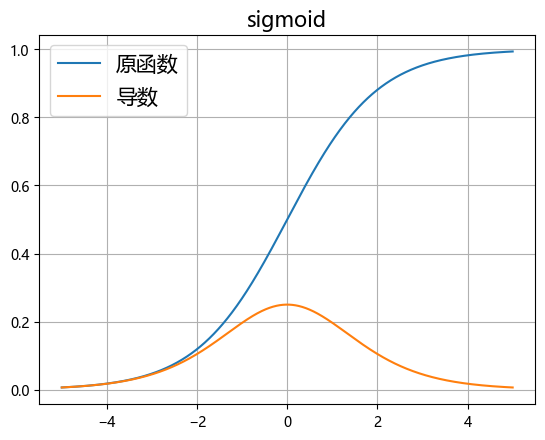
\includegraphics[width=0.45\textwidth]{figures/sigmoid函数和导数.png}}
    \subfigure[tanh]{
    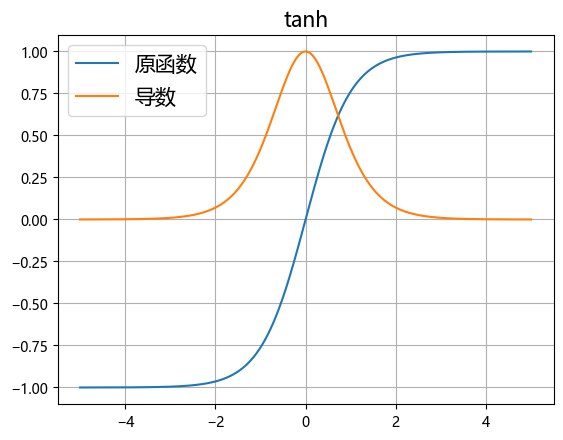
\includegraphics[width=0.45\textwidth]{figures/tanh.png}}
    \subfigure[ReLU]{
    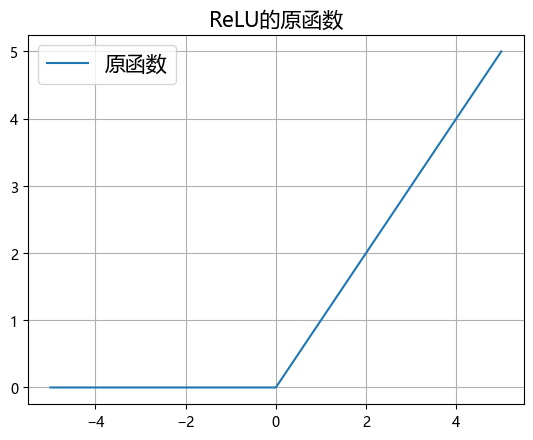
\includegraphics[width=0.45\textwidth]{figures/ReLU图像.png}}
    \subfigure[Leaky ReLU]{ \label{Leaky relu}
    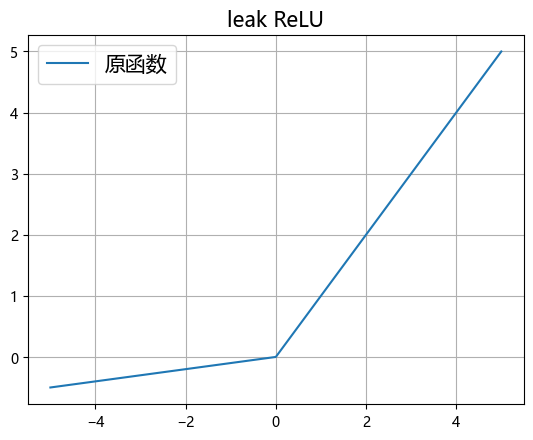
\includegraphics[width=0.45\textwidth]{figures/Leaky ReLU.png}}
    \caption{不同激活函数的原函数和导数}
\end{figure}
\newpage

\section{神经网络代码实现}

现在神经网络框架的集成程度已经相当高,只需要简单几行代码就可以建立一个简单的神经网络。常用的框架有Pytorch,Tensorflow和Keras等,其中Keras已经被集成到Tensorflow。读者只需要选一个框架学习即可,这里推荐Pytorch,因为其社区支持很好,学术界也普遍采用该框架,但笔者目前主要使用Tensorflow。注意,学习本节需要读者对python编程有一定的掌握,并且要熟悉numpy,matplotlib等重要包的使用。

\subsection{现成框架调包实现}

每个框架都有多种写法,这里仅展示比较简单,便于理解的进行展示,你需要综合你前面全部所学去理解这些代码,因此有一定难度,但仍然推荐看看如何用现成框架实现,尽管不推荐重复造轮子,但最好知道轮子的原理。

\subsubsection{回归/拟合任务}

\begin{table}[ht]
    \centering
    \begin{tabular}{c c c c}
      index & 模拟考试A & 模拟考试B & 期末考试  \\ \hline
         1  & 85     &   76     &  80      \\ 
         2  & 76     &   83     &  80      \\ 
         3  & 90     &   86     &  87      \\
         4  & 70     &   80     &  73      \\
         ...&  ...   &   ...    &  ...
    \end{tabular}
    \caption{成绩单}
\end{table}

一般的回归任务,例如对表格\ref{table1}来说,需要拟合期末考试分数,输入的是前两次模拟考试的分数,大小为2,那么应该提前准备好\verb|x_train|,它包含前面两个字段\footnote{对于任何即将倒入神经网络的数据来说,都不要专门包含一个index字段,这里只是模仿excel软件中的显示方便阅读},同样的\verb|y_train|就包含最后一个字段“期末考试”。我还单独准备了验证集数据\verb|x_valid, y_valid|,也可以不手动准备,参考下一节分类任务\ref{分类任务}代码。验证集的作用是方便调整参数,例如神经元层数或者个数,因为我们用训练集进行训练,要验证它的效果,就需要在一个同分布的陌生的数据中去测试,验证集和测试集来源于同一个数据,因此它们的分布是一样的,此外还有测试集,有时候可以不用准备,因为测试集相当于在实际问题中应用模型,有时候我们只需要评估效果,用验证集就够了。关于如何整理表格并且分字段赋值到另一个变量中,请参考\verb|pandas|包的文档。

\begin{python} \label{回归任务代码}
# 基于tensorflow实现
import tensorflow as tf
from tensorflow import keras
model = keras.models.Sequential([
    keras.layers.Dense(30, activation="relu", input_shape=[2]),
    # 第一层30个神经元,激活函数ReLU,输入神经元8个,输入层大小2
    keras.layers.Dense(20, activation="sigmoid"),
    # 第二层20个神经元,激活函数sigmoid
    keras.layers.Dense(1)
    # 最后一层输出层,1个神经元,没有激活函数
])
model.compile(loss="mse", optimizer=keras.optimizers.SGD(learning_rate=1e-3))
# 编译模型,损失函数为mse,优化器为SGD,其中学习率0.001
history = model.fit(x_train, y_train, epochs=10,
                    validation_data=(x_valid, y_valid))
# 训练模型,输入x_train y_train,训练10个迭代,验证数据集为x_valid, y_valid
\end{python}

在\verb|model|的最后一层有一个神经元没有写激活函数,因为在回归或者拟合任务中,输出就是一个值,需要拟合的是期末考试成绩,只是一个值,如果在最后一层采用$sigmoid$激活函数,那么输出就在0到1之间,这不符合现实,或者加一个$ReLU$,小于0的输出将直接变成0,在本例中成绩分数一定大于等于0,但是在其他任务中则完全有可能小于0,不必多此一举。

训练模型的命令是model.fit(),输入x和y,模型会自动依据这两个数据进行优化,比如梯度下降,这里还有其他参数,可以参考相关文档。

\subsubsection{分类任务}\label{分类任务}

我们虚构一个分类任务,现在有三个特征和一个标签,“花的种类”有四种,用1,2,3,4来表示,那么同样的\verb|x|应该是包含前三个字段的表格,\verb|y|包含“花的种类”,这里没有单独划分验证集,而是在函数\verb|fit()|中指定\verb|validation_split=0.3|,表示输入的数据中有30\verb|%|用于验证。

\begin{table}[ht]
    \centering
    \begin{tabular}{c c c c c}
      index & 花瓣长度 & 花瓣宽度 & 锯齿深度 & 花的种类  \\ \hline
         1  & 23     &   12     &  2      &   2     \\ 
         2  & 12     &   5      &  0.5    &   1     \\ 
         3  & 32     &   25     &  5      &   4     \\
         4  & 70     &   35     &  9      &   3     \\
         ...&  ...   &   ...    &  ...    &  ...
    \end{tabular}
    \caption{花种分类}
    \label{table2}
\end{table}

\newpage

\begin{python}
# 基于tensorflow实现
import tensorflow as tf
from tensorflow import keras
model = keras.models.Sequential([
    keras.layers.Dense(30, activation="relu", input_shape=[3]),
    # 输入的大小是3,对应三个特征
    keras.layers.Dense(20, activation="sigmoid"),
    keras.layers.Dense(4, activation="softmax")
])
model.compile(loss="sparse_categorical_crossentropy", optimizer='nadam', metrics=["accuracy"])
# 编译模型,损失函数为二元交叉熵,优化器为nadam
history = model.fit(x, y, epochs=10,
                    validation_split=0.3)
\end{python}

\begin{equation}
    softmax(x_i) = \frac{e^{x_i}}{\sum^{n}_{j=1}{e^{x_j}}}
\end{equation}

最后有4个神经元输出,激活函数用$softmax$,这是$sigmoid$的多分类改进,它们的输出区间是一样的,都是(0,1),分子是全部分母中的一个,这里有四个分类,因此$n=4$,一共有四个分母。模型输出的是4个在(0,1)区间的一维张量,里面每个数代表一个分类的概率,表明属于该分类的概率。此外损失函数也变成了二元交叉熵而非mse,这是分类任务的损失度量方法,优化器变成nadam,这是现在最先进的梯度下降方法之一,我们还加了个衡量标准"accuracy",你暂时不需要了解太多这些新知识,先学会使用和观察效果即可。

\subsection{纯手搓神经网络}

我们需要引用下面的包,如果你没有这些包,则需要在终端中键入命令:
pip install numpy,以此类推。
\begin{python}
import numpy as np
import pandas as pd
import matplotlib.pyplot as plt
\end{python}

先准备数据,在-2到2之间等距取1000个x点,y=2sinx,并且在y上加一些噪声,同时还要给x和y加一个维度。
\begin{python}
x0 = np.linspace(-2, 2, 1000)
y0 = 2 * np.sin(x0)
y0 += 0.32 * np.random.randn(y0.shape[0]) # 加噪声

x = x0[:, np.newaxis]
y = y0[:, np.newaxis]
\end{python}

写一个loss函数度量损失,只要输入一个或一组预测y值,再输入一个或一组真实y值,此函数返回$mse$值。

\begin{python}
def mse(yl, y0):
    return ((yl - y0)**2).sum()/yl.shape[0]
\end{python}

我们用统计学的最小二乘法,也就是公式法,求出线性回归的函数,以此作为baseline,在机器学习领域经常需要建立一个基准,以验证模型是否存在改进。

\begin{python}
b2 = float((len(y0)*(x0*y0).sum(0) - y.sum(0)*x0.sum(0)) /
           (len(x0)*(x0**2).sum(0) - (x.sum(0)**2)))
b1 = float(y0.mean() - b2 * x0.mean())
print('回归方程为: y = {:.2f} + {:.2f} * x'.format(b1, b2))
# 数据是标准化的,因此截距项为0
\end{python}
\verb|回归方程为: y = 0.01 + 1.31 * x|

画出最小二乘法给出的函数图像
\begin{python}
yl = []
for i in x0:
    yl.append(b1 + b2 * i)
yl = np.array(yl)
plt.scatter(x0, y0, label='原始点')
plt.plot(x, yl, 'r', label='最小二乘法回归线, 损失{:.3f}'.format(baseline))
plt.legend(fontsize='13')
\end{python}

\begin{figure}[h]
    \centering
    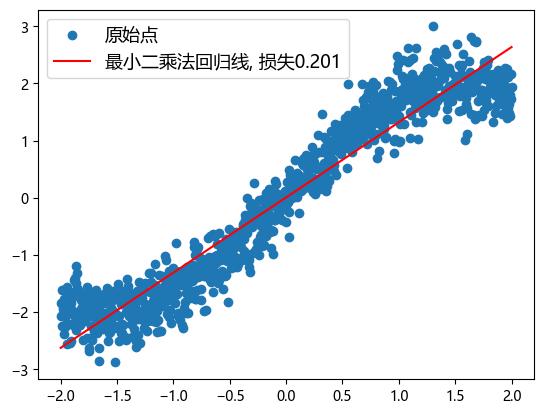
\includegraphics[width=0.5\textwidth]{figures/最小二乘法图像.png}
\end{figure}

我们再用Keras来训练一下,其结构与我后面手搓的神经网络一致,即一个隐藏层,包括5个神经元,输出层有1个神经元。

\begin{python}
from tensorflow import keras
model_tf = keras.models.Sequential([ 
    keras.layers.Dense(5, input_shape=[1,], activation='sigmoid'),
    keras.layers.Dense(1),
])
model_tf.compile(loss='mse', optimizer=keras.optimizers.SGD(0.01))
history = model_tf.fit(x, y, epochs=50, validation_split=0.3)
# 用百分之三十的数据作为验证集,每次迭代会被自动打散并且分割数据

pd.DataFrame(history.history).plot(figsize=(8, 5)) # 画出损失图像
# 画出对比图象
plt.scatter(x0, y0, c='gray', label='原始点')
plt.plot(x0, yl, 'r', label='最小二乘法回归线, MSE为 {:.3f}'.format(baseline))
plt.plot(x0, y_tf, 'green', label='keras神经网络, MSE为 {:.3f}'.format(keras_mse))
plt.legend(fontsize='10')
\end{python}

得到下面两张图,左边是损失情况,其中橙色的线是验证损失,蓝色的是训练损失,具体含义在\ref{评价方法}详细解释,右边可以看到黄色线是Keras的训练结果。

\begin{figure}[ht]
    \centering
    \subfigure[损失情况]{
    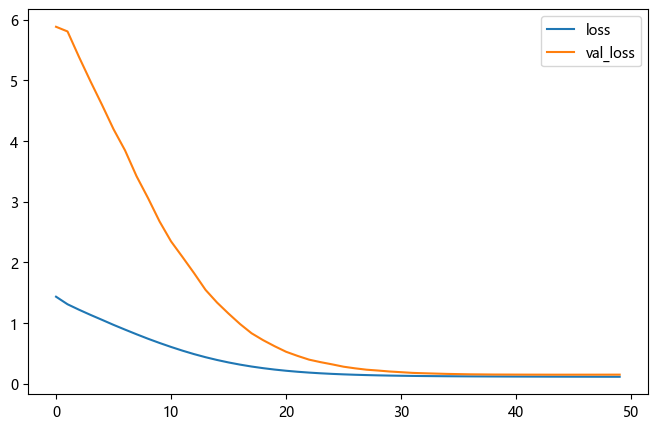
\includegraphics[width=0.5\textwidth]{figures/损失情况.png}}
    \subfigure[对比图像]{
    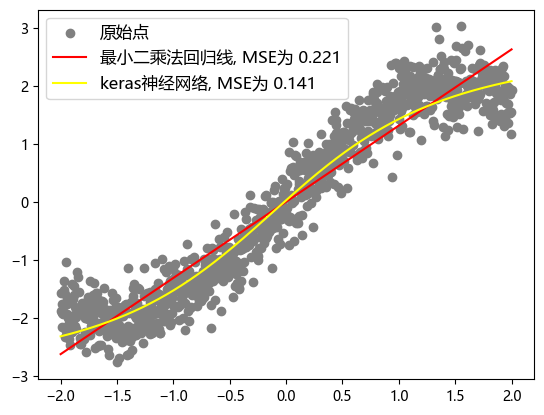
\includegraphics[width=0.45\textwidth]{figures/对比图象.png}}
    \caption{状态1}\label{状态1}
\end{figure}



下面是手搓神经网络的完整代码,如果还没有学类封装编程,可以先跳过。由于实现神经网络的类的代码比较长,书中排版显示的代码不一定美观,因此我只放截图避免过多空间占用,原代码可以通过前言中提供的链接\ref{代码链接}在线浏览\href{https://github.com/Aegis1863/ML_practice/blob/master/机器学习笔记/X_01_手搓BP神经网络.ipynb}{<手搓BP神经网络>}。

\newpage

\begin{figure}[h!]
    \centering
    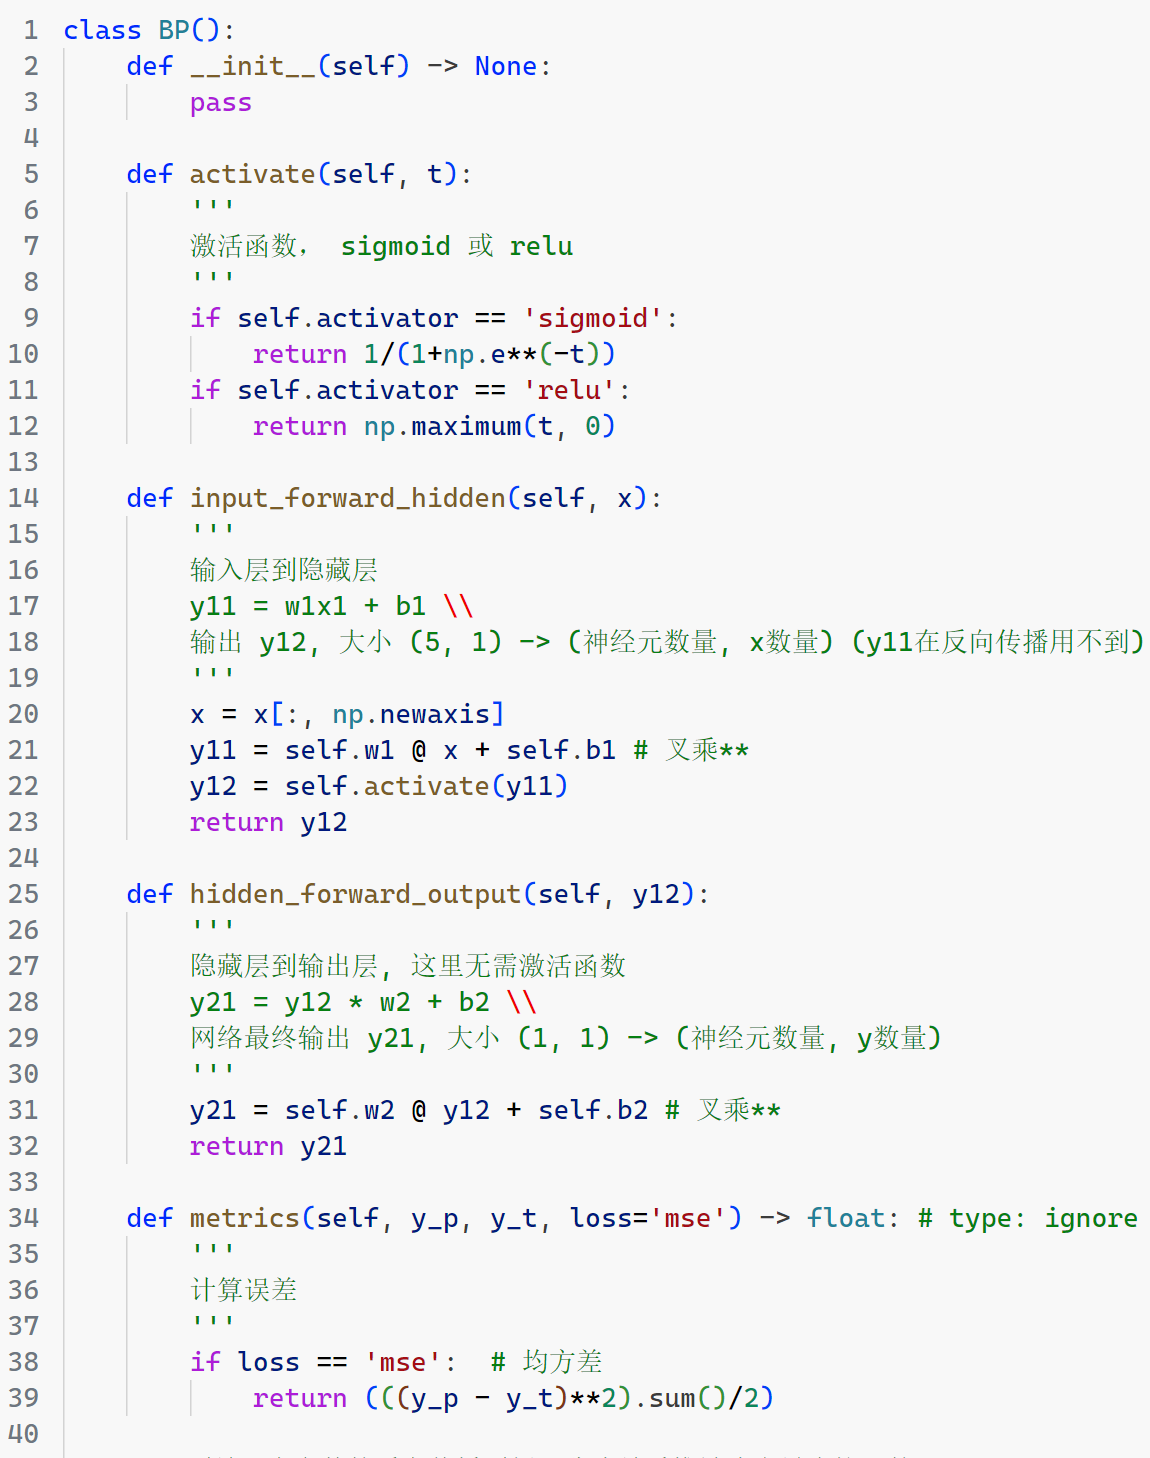
\includegraphics[width=\textwidth, frame]{figures/BP1.png}
\end{figure}

\newpage

\begin{figure}[h!]
    \centering
    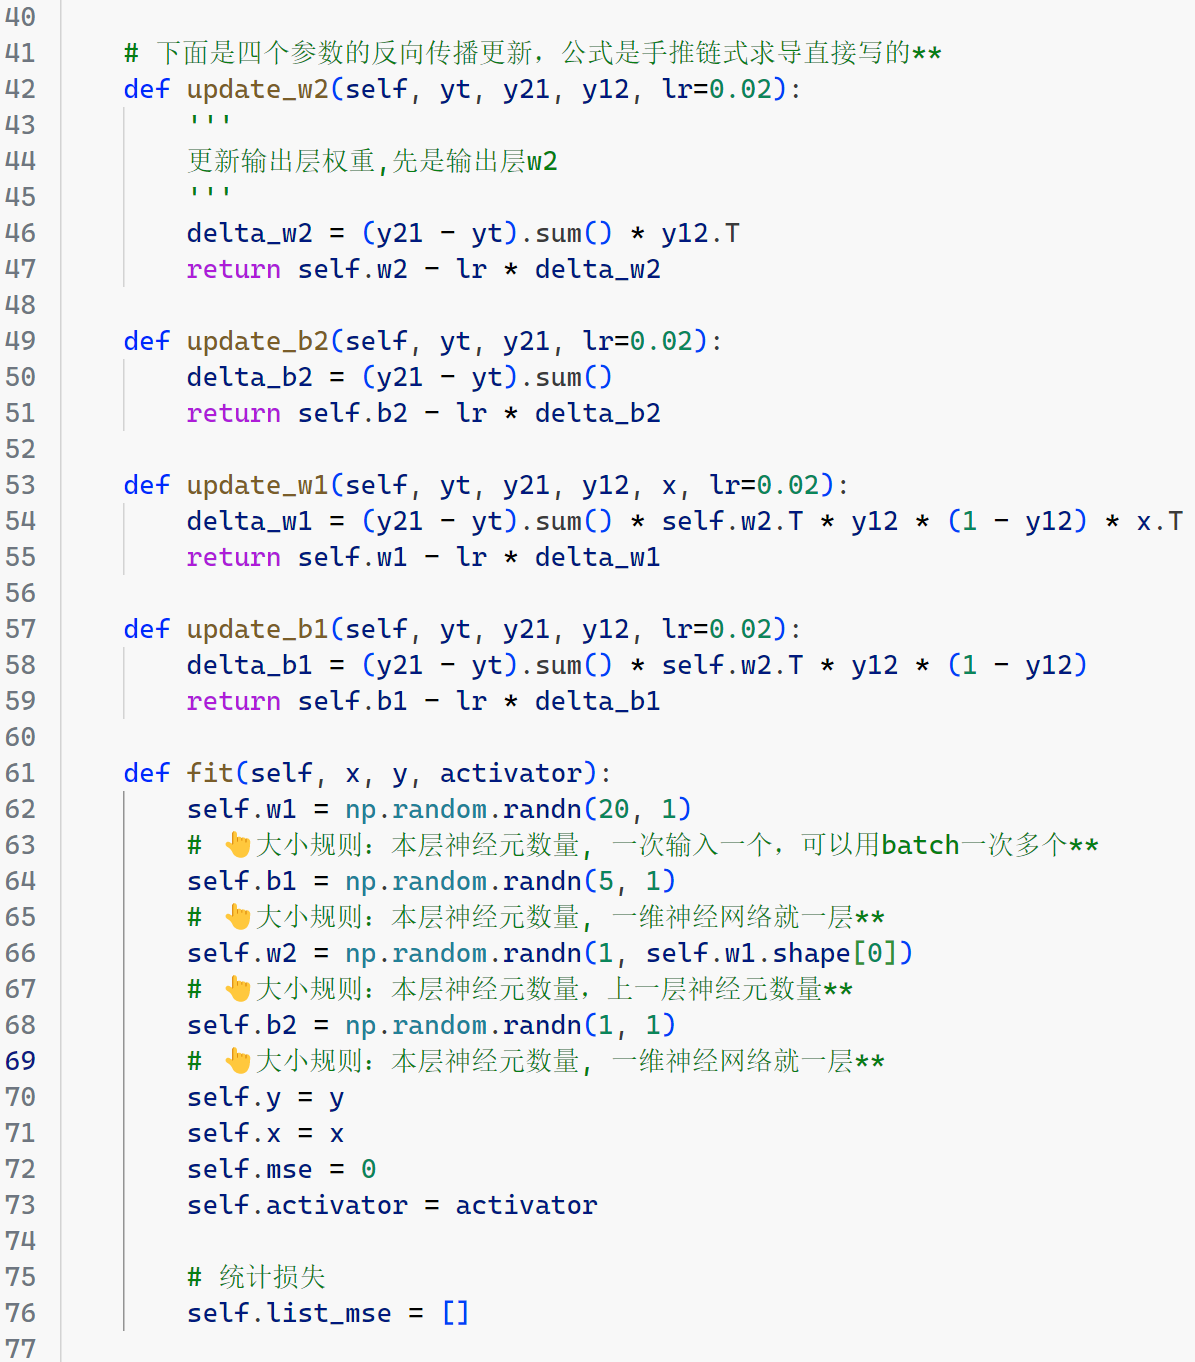
\includegraphics[width=\textwidth, frame]{figures/BP2.png}
\end{figure}

\newpage

\begin{figure}[h!]
    \centering
    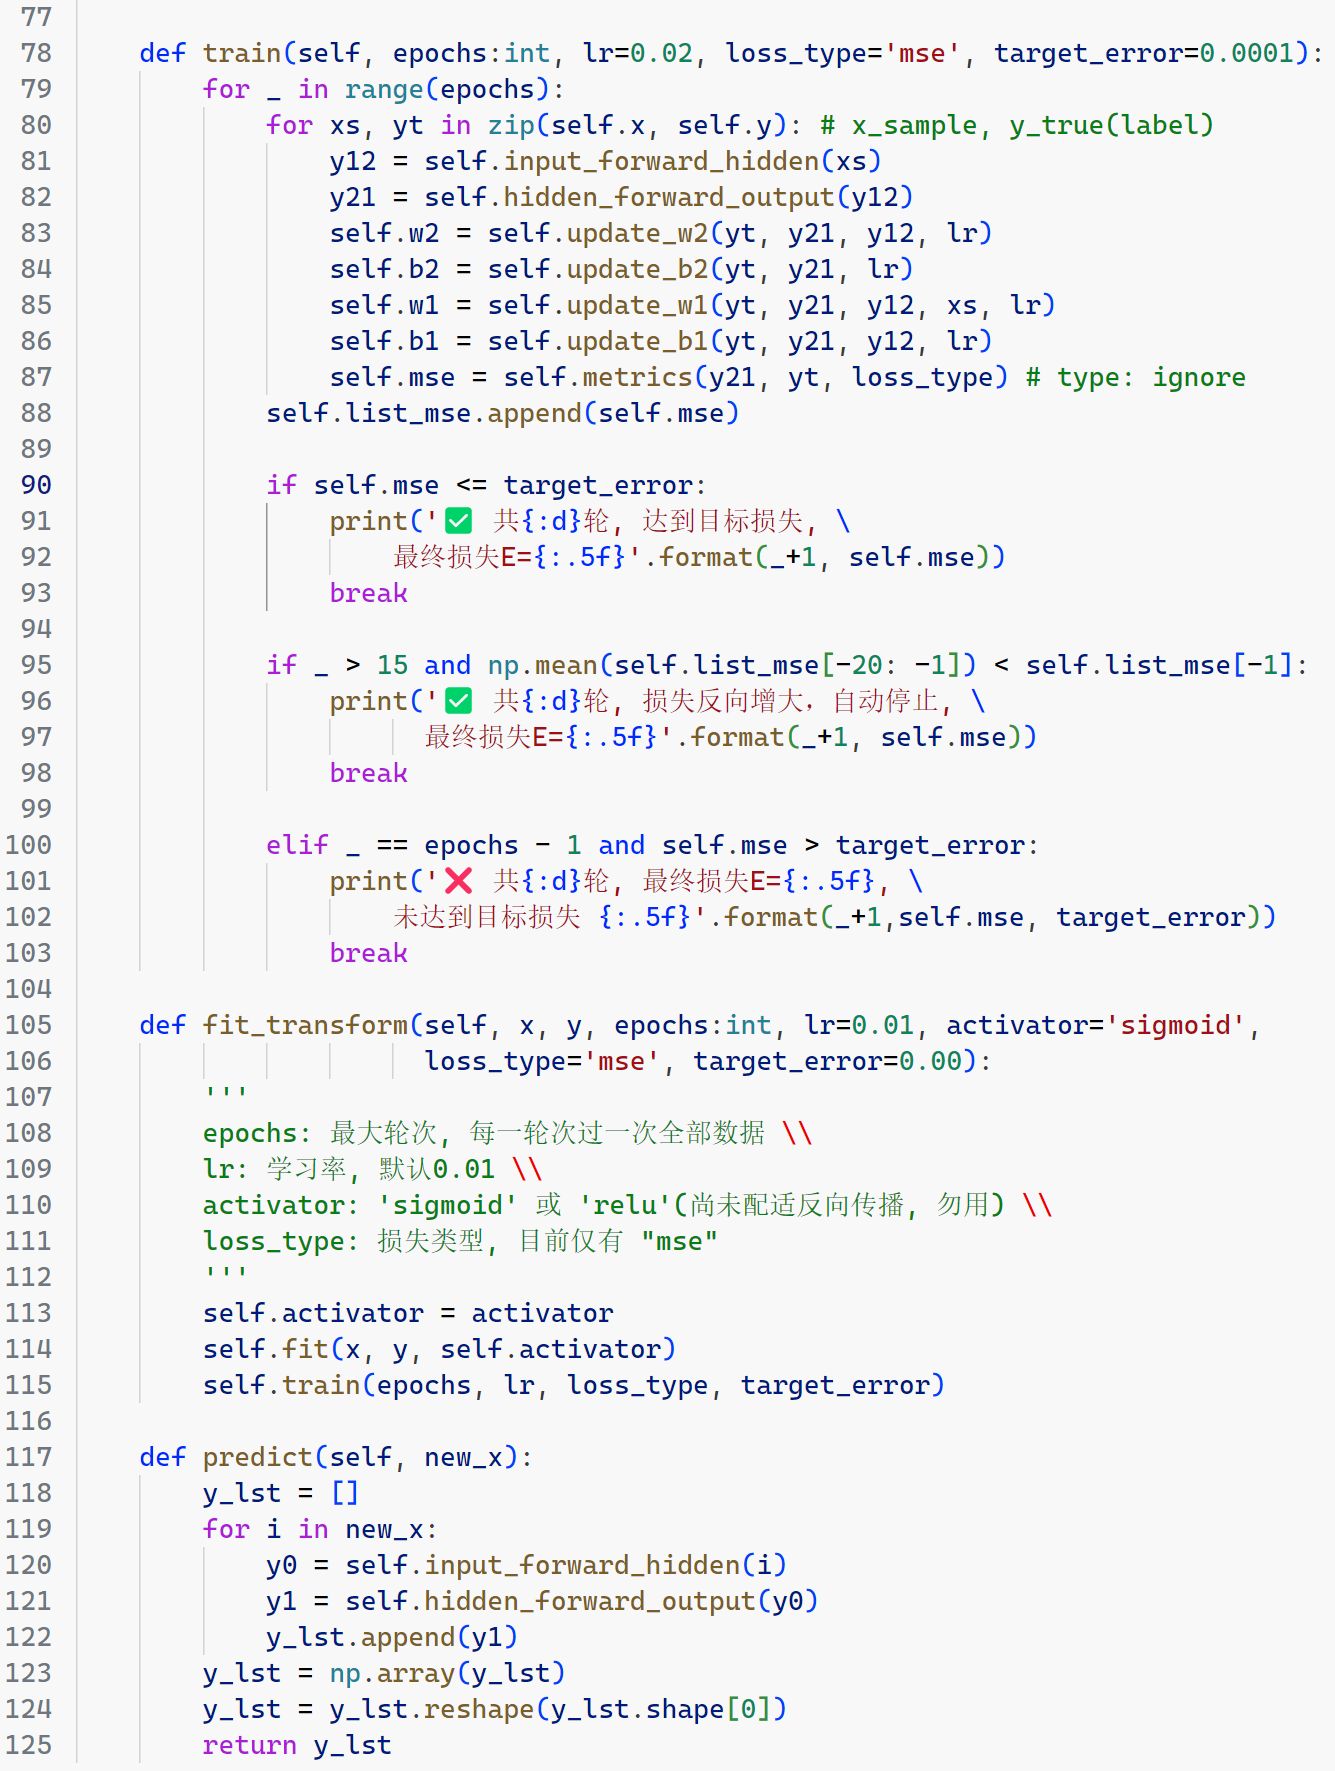
\includegraphics[width=\textwidth, frame]{figures/BP3.png}
    \caption{代码图片}\label{代码图片}
\end{figure}

\newpage

调用并且训练此类:

\begin{python}[h]
model = BP()
model.fit_transform(x, y, 100, lr=0.0005, activator='sigmoid')
\end{python}

\verb|√ 共28轮, 损失反向增大,自动停止, 最终损失E=0.00238|

查看损失情况和对比图:
\begin{python}
plt.title('损失情况', fontsize=15)
plt.ylabel('损失', fontsize=15)
plt.xlabel('训练回合', fontsize=15)
plt.grid()
plt.plot(model.list_mse, label='神经网络')
yp = model.predict(x)
plt.text(0, -2.5, 'y=2sinx', fontsize=15)
plt.scatter(x, y, s=3, c='gray', label='原散点')
plt.plot(x0, yl, 'r', label='最小二乘法回归线, mse = {:.3f}'.format(baseline))
plt.plot(x0, y_tf, 'green', label='keras神经网络, mse = {:.3f}'.format(keras_mse))
plt.plot(x, yp, c='b', label='手搓神经网络, mse = {:.3f}'.format(bp_mse))
plt.legend(fontsize=10)
\end{python}

\begin{figure}[h!]
    \centering
    \subfigure[损失情况]{
    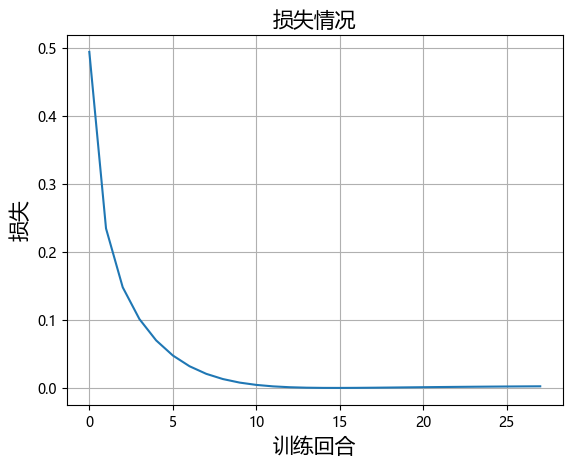
\includegraphics[width=0.46\textwidth]{figures/损失情况2.png}}
    \subfigure[对比图像]{
    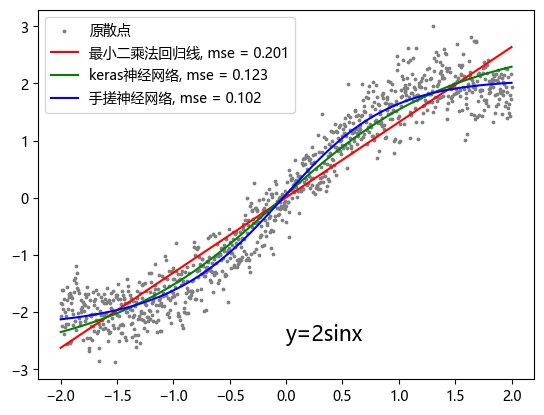
\includegraphics[width=0.48\textwidth]{figures/对比图象2.png}}
    \caption{状态2} \label{状态2}
\end{figure}

与图\ref{状态1}类似,图\ref{状态2}左边表示损失变化的情况,但我没有实现展示验证集损失的效果,右边是三种方法的拟合对比图,可以看到蓝色线条表示的手搓神经网络的拟合效果是不错的。你还可以检查一下我的\verb|update_w1()|等函数是否与前面的偏导公式\ref{偏导}一致,位置在上面的代码图片\ref{代码图片}的45行至62行。

我没有对整个手搓代码进行详细的分段解释,这里仅作一些提示,比如激活函数是需要定义好的,误差函数也可以方便地引用,有点类似于搭积木,如果你很熟悉神经网络所需的各个部件,那么你就自然而然地想写出每一个部件的函数,这个思路是没错的,但是如果仔细看我网络的实现方法,例如\verb|input_forward_hidden()|,会发现我只是在里面进行张量计算,而不是“定义5个实际的神经元函数”,也许这也行得通,但我没有尝试过,我也并不是算法天才QAQ。在我的框架中,要改变神经元数量需要在\verb|fit()|方法中进行修改,而且不方便修改层数,反向传播写的是硬代码\footnote{定义见\ref{硬代码解释}}而非自动微分技术。

自己写神经网络是需要花不少功夫的,很多人在短时间内就可以理解神经网络的原理,但是真的动手时会发现很多问题,代码会出现很多bug,都需要自己一遍又一遍调试,我直到基本学完深度学习基础之后才回过头来尝试手写神经网络代码,本以为应该是得心应手,毕竟调包的时候手到擒来,但实际上困难重重,你需要对每一个细节进行把关,任何一个理解错误都可能导致整个模型功亏一篑,同时,这也是对你编程能力的重要挑战。

%%%%%%%%%%%%%%%%%%%%%%%%%%%%%%%%%%%%%%%

\chapter{机器学习效果评估} \label{评价方法}

\section{一般情况}

在现成的机器学习框架中,一般都比较友好地给出了模型返回的一些数据,并且可以方便地作图。此外也可以采用F1分数,PR图像或者AUC图像来衡量模型质量,但是它们通常用于传统机器学习中,在深度学习领域比较少见,因此不在这里介绍。

在前面的机器学习任务代码中,如果我们在后面运行命令:

\begin{python}
pd.DataFrame(history.history).plot()
plt.grid(True)
plt.gca().set_ylim(0, 1)
plt.show()
\end{python}

大概会得到类似下面的图像,$loss$是训练损失,$val\_loss$是验证损失,$loss$降低或$accuracy$增加就是比较正常的,这些指标最终会趋于稳定。

\newpage

\begin{figure}[h]
    \centering
    \subfigure[回归任务]{
    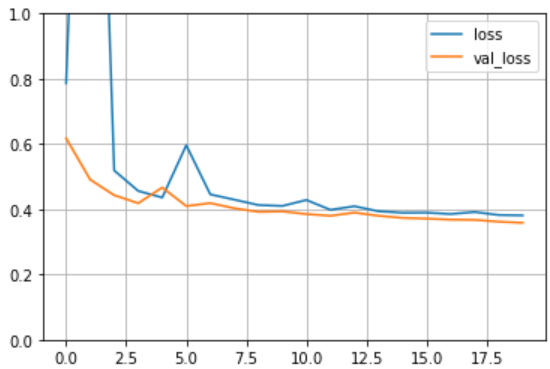
\includegraphics[width=0.47\textwidth]{figures/回归任务图像.png}}
    \subfigure[分类任务]{
    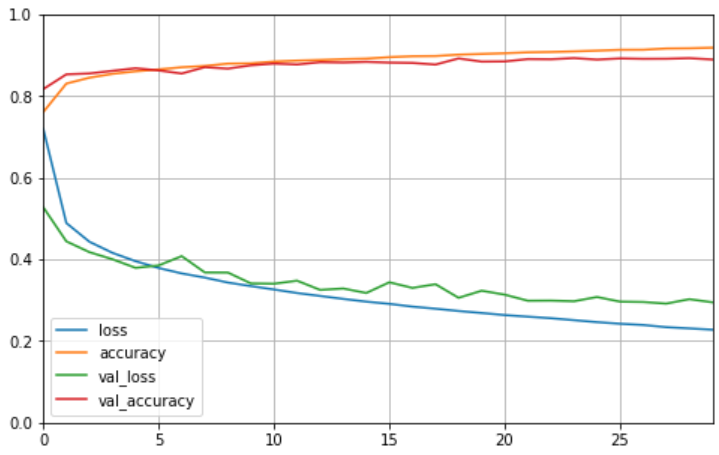
\includegraphics[width=0.49\textwidth]{figures/分类任务图像.png}}
    \caption{两种任务的结果可视化}
\end{figure}

\section{损失曲线剧烈震荡}
有时候会出现剧烈震荡,很有可能是因为学习率太大,例如要从5调整到4,但是学习率比较大,导致一次修改10,那么就永远不会收敛到4,误差也就一直震荡下去。

\section{过拟合和欠拟合}
如果验证损失明显大于训练损失,说明模型过拟合了,在\ref{figure3}中,我们只需要一条大致的直线或者s型曲线来拟合数据,而不需要构造一条线穿过所有的点,如果过拟合了,建议减少神经元个数和层数,也可以用特殊方法调整权重的初始化值,这些方法可以在Pytorch或者Tensorflow的文档中找到\footnote{对于新手来说看文档是有一定困难的,但是建议养成这个习惯,你也可以利用搜索引擎直接搜索相关方法}。如果$loss$比较大,说明欠拟合,也就是效果不佳,你可以增加神经元个数和层数。

\section{确定基准}
如何判断$loss$是大是小呢,这就需要添加一个基准,例如在\ref{figure3}中,基准是用最小二乘法回归的一条直线,在二分类任务中,就算我们盲猜结果,大约也会获得0.5的正确率,因此0.5就是基准,如果模型的准确率接近0.5,那就说明没有起到优化的作用。

\section{调整图像}

训练集的结果与验证集不是完全同步的,验证集是在测试集之后做的验证,它们在同一个迭代中,因此可以说验证集的$val\_loss$或$accuracy$比测试集的要晚半个回合,通常我们不会做特殊处理,即把测试集数据前移半个回合,但你也的确可以做特殊处理。



%%%%%%%%%%%%%%%%%%%%%%%%%%%%%%%%%%%%%%%

\chapter{模型改进技术}

有很多方法可以在基本模型的基础上进行调整改进,比如$Glorot$和$He$权重初始化,之前提到过,我们最开始初始化$w$和$b$只是在正态分布中随机取值;可以改激活函数,比如$ReLU$改$Leaky~ReLU$或者别的;还可以批量归一化、梯度裁剪、迁移学习、用更好的优化器如$adam$、正则化、dropout等,这里只介绍几个常用的,其他的方法读者可以自行学习其他资料。

\section{批量归一化}

归一化也就是标准化,英文简称BN(Batch Normalization),与统计学中的概念一致,但是不要问我为什么$\sigma^2$里面用$\frac{1}{n}$而不是$\frac{1}{n-1}$...

$\mu = \frac{1}{n}\sum^{n}_{i=1}x_i$ 

$\sigma^2 = \frac{1}{n}\sum^{n}_{i=1}(x_i-\mu)^2$

$\hat{x_i} = \frac{x_i-\mu}{\sqrt{\sigma+\epsilon}}$ 

$z_i = \gamma\otimes\hat{x_i}+\beta$

在第三个式子标准化x时,分母加了一个$\epsilon$,是为了避免分母取到0而报错,$\epsilon$可以给一个很小的值例如0.001。批量归一化的意思就是一次取一个批量的数据进行归一化,比如一次取32个,在Keras中会默认这个参数,也可以手动调整,太大的批量会导致运算过慢,太小的批量会导致资源空闲。如果在模型最开始做一个归一化,那么相当于对数据进行了预处理。此外,层归一化增加了模型参数,比如上面公式中的$\gamma$和$\beta$,它们用来缩放调整图像,这也是需要梯度下降的,会使得模型的复杂度增加。

在代码构建中,这一步非常简单,只需要加一个\\
\verb|BatchNormalization()|

\begin{python}
model = keras.models.Sequential([
    keras.layers.Flatten(input_shape=[28, 28]),
    keras.layers.BatchNormalization(),  
    # 每一层中间都加一个批量归一化
    keras.layers.Dense(300, activation='relu'),
    keras.layers.BatchNormalization(),
    keras.layers.Dense(100, activation='relu'),
    keras.layers.BatchNormalization(),
    keras.layers.Dense(10, activation='softmax')
])
\end{python}

批量归一化在计算机视觉中经常使用,这种技术通常可以把基本模型的精度再提高几个点。

在最先进的技术,比如Transformer构架中,作者把批量归一化改成了层归一化,即对每一个样本自身进行归一化,而不是对若干个样本的特征归一化,在这里不详细说明。

\section{dropout}

在传统机器学习中,正则化通常使用$l_1$或$l_2$范数,但是在深度学习中,最常用的是dropout,它是由"深度学习之父"Geoffrey Hinton在2012年的论文中提出的\footnote{Geoffrey E. Hinton et al., "Improving Neural Networks by Preventing Co-Adapation of Feature Detectors," arXiv preprint arXiv:1207.0580(2012).},只要使用该技术,即便是最先进的模型也能进一步提高1~2\%的精确度。

dropout就是在每次训练中随机关闭一些神经元,比如关闭30\%,假如公司规定每天都随机有一些人休息不上班,那么就会空缺一些岗位,剩下的员工就必须尝试兼职那些空缺的岗位,并且加强合作效率,这是对dropout产生更好效果的一个比喻,是的只是一个比喻,关于神经网络或者神经元为什么会这样或者那样运作,至今也没有定论,这也就是神经网络的难以解释的特性。通过添加该方法,你的神经网络会更鲁棒\footnote{碰到特殊情况也能够较好的处理},有更好的泛化能力。

在代码中也很容易实现,只需要用Dropout()方法,传入一个丢弃率:

\begin{python}
# 使用0.2的dropout率在每个Dense层之前应用dropout正则化,它将丢弃一些输入,将剩下的输入传递到下一层

model = keras.models.Sequential([
    keras.layers.Flatten(input_shape=[28, 28]),
    keras.layers.Dropout(rate=0.2),
    keras.layers.Dense(300, activation='elu'), 
    keras.layers.Dense(100, activation='elu'),
    keras.layers.Dropout(rate=0.2),
    keras.layers.Dense(10, activation='softmax')
])
\end{python}

\newpage

\section{残差连接}\label{残差连接}

这是卷积神经网络中常用的技术,也是划时代的技术,由何凯明、张弛、孙剑等人提出\footnote{Kaiming He et al., "Deep Residual Learning for Image Recognition", arXiv preprint arXiv:1512:03385(2015)},也可以用在普通神经网络中,其结构非常简单,但构建起来会稍微复杂一点。

\begin{figure}[h!]\label{残差连接图像}
    \centering
    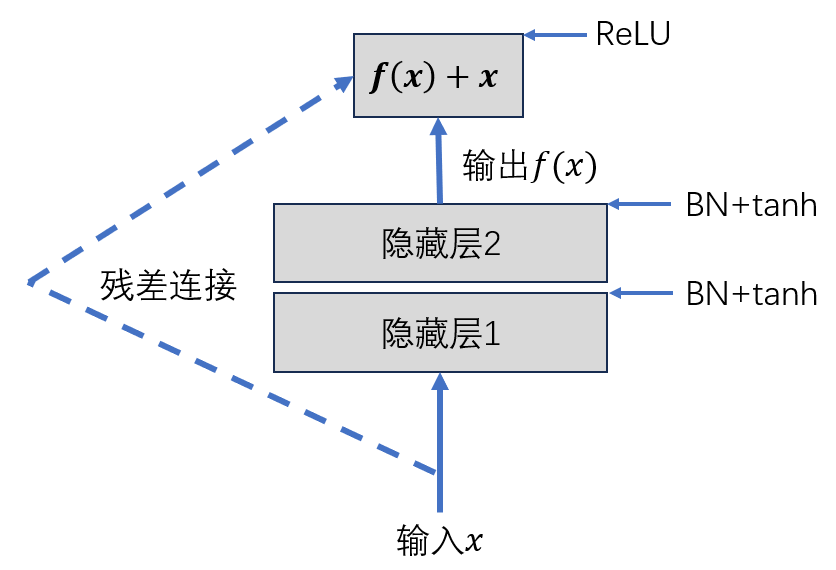
\includegraphics[width=\textwidth]{figures/残差单元.png}
    \caption{残差连接}
\end{figure}

BN表示批量归一化,ReLU和tanh表示激活函数,在图\ref{残差连接图像}中,输入x通过两个隐藏层之后输出$f(x)$,此时再加上初始输入的x,于是输出的是$f(x)+x$,这个改进看起来相当简单,然而的的确确是划时代的改进。

之前提到过梯度消失问题,如果我们用sigmoid激活,层数很大时,梯度累乘可能导致梯度消失影响训练效率,在卷积神经网络中,通常用tanh激活函数,也不能避免梯度消失问题,但是一旦把输出改成$f(x)+x$,其导数就是:

\begin{equation}
    \frac{\partial{(f(x)+x)}}{\partial{x}} = \frac{\partial{f(x)}}{\partial{x}} + 1
\end{equation}

就算f(x)的梯度很小,这个偏导也是接近1的,从而避免了梯度消失问题。在机器学习中,即便是一个简单的创新,只要对模型有提升,也是划时代的贡献。

\subsubsection{代码构建}

代码涉及到继承的方法,如果看不懂可以先跳过,\href{https://github.com/ageron/handson-ml2/blob/master/14_deep_computer_vision_with_cnns.ipynb}{<代码修改自以下链接,第33个代码块>}
\begin{verbatim}
https://github.com/ageron/handson-ml2/blob/master/
14_deep_computer_vision_with_cnns.ipynb
\end{verbatim}

\begin{python}
class ResidualUnit(keras.layers.Layer):
def __init__(self, filters, strides=1, activation="relu", **kwargs):
    super().__init__(**kwargs) # 继承父类参数
    # 激活函数默认ReLU
    self.activation = keras.activations.get(activation)
    # 构建两个隐藏层,合并作为主要层,中间有两个BN层
    self.main_layers = [
        keras.layers.Dense(10, self.activation, 
                            input_shape=[3]),
        keras.layers.BatchNormalization(),
        keras.layers.Dense(20, self.activation)
        keras.layers.BatchNormalization()]

def call(self, inputs):
    Z = inputs # 输入的x赋值给Z
    # 让Z经过主要各层,最后Z等于前面图片中的f(x)
    for layer in self.main_layers:
        Z = layer(Z)
    # skip_Z等于我们最开始给的x
    skip_Z = inputs
    return self.activation(Z + skip_Z) # 实现残差连接
\end{python}

%%%%%%%%%%%%%%%%%%%%%%%%%%%%%%%%%%%%%%%


\chapter{磨练技术的途径}

\section{kaggle竞赛}

kaggle官网:\href{https://www.kaggle.com/}{kaggle官网}\footnote{https://www.kaggle.com/},kaggle是被谷歌公司收购的机器学习竞赛平台,几乎每个时期都有各类大小型比赛,并且提供大量数据,有些竞赛是由其他公司赞助的,并且提供高额奖金。

我在学习传统机器学习时期在kaggle中参与了一些简单的竞赛,比如泰坦尼克号数据集,简单比赛的数据清洗难度比较低,经过一定的加工就可以在大部分机器学习模型中运行,非常适合锻炼代码能力和构建机器学习模型的熟练度。在每个竞赛中,只要你按要求提交了一个结果,就会得到一个总排名,可以看到你和其他人模型的得分,还可以看到其他人的成绩和他们的解决方案,比如代码笔记本,你可以找到得分最高的人并且学习他们的实现方法。

由于kaggle是全英文的,你可能会需要用到翻译软件,但如果花一点精力,其实能够看懂大部分英文信息,这同样是锻炼英文能力的好地方。

\section{数学建模国赛}

数学建模中大数据题的热度越来越高,几乎每年都有一个数据分析的题目,当然也会有其他类型的题目,比如涉及到博弈论或者动态规划问题的,我对2013年的B题进行了练习,给出了解决方案,但并不是基于机器学习的,读者可以参考一下\href{https://github.com/Aegis1863/Problem-of-splicing-paper-fragments}{碎纸片拼接问题}\footnote{https://github.com/Aegis1863/Problem-of-splicing-paper-fragments}。

此外,我参与了2020年数学建模国赛的C题,主办方提供了一些银行借贷的特征数据,其中包含一个“是否借贷”的字段,显然需要我们进行机器学习,题目要求参赛组对借贷情况进行数据分析,并且给出一个借贷策略,我们小组在制定策略方面采用了神经网络方法,即用一些借贷数据的特征预测是否要借贷。

然而神经网络在数学建模竞赛中并不被推崇,至少在2020年以前是那样,因为深层神经网络的可解释性非常差,机器学习不只有神经网络,如果用传统机器学习方法,构建logistic回归模型,那么可解释性当然是更强的,这在数模竞赛中更有优势,此外特征工程也是一个非常重要的任务,例如要预测房价,只给一个地区的人口和房屋总数,也许有一定效果,但是如果建立一个新特征,比如人口除以房屋总数,也就是人均房屋数,它与房价的相关程度可能更高,模型也就有更好的效果。

特征工程属于数据清洗之后的一个可选步骤,本书中没有详细提及数据清洗和特征工程。推荐读者学习北京理工大学嵩天的视频课程\ref{视频课程}。

我的小组在那次比赛中获得了省一等奖,实际上,在那之前,神经网络方法获得省一也是很少见的,因为低解释性的原因,事后认为可能是因为我们组做了大量特征工程,这一点比较契合办赛宗旨。

数学建模国赛在每年的九月初,读者若想参与,在读期间,可以在开赛前任意时间报名,如果想冲刺国奖,三位组员都需要有良好的科研素质和科研能力。推荐三人组队分工:模型构建者、程序员、论文撰写者。其中程序员时间会很紧张,需要大量连续的时间写代码,模型构建者的任务,狭义来说就是负责构建公式,如果也具备代码能力,可以协助编程,论文撰写者的任务也就是字面意思,最好是熟悉论文撰写并且有较多经验的同学负责。三个组员也要对其他人的任务有一定的了解,不能完全割裂,竞赛只有三天时间,需要良好的配合。

最后补充一点,数学建模竞赛并不是“深度学习”竞赛,你还需要大量其他的工作,比如分析问题,解释问题和模型等。

\section{自己练习}

自己练习也是很重要的,你可以在学习的过程中随时尝试用已经学到的方法应用在一个新的数据上,尝试写一些小程序。

在我的机器学习\href{https://github.com/Aegis1863/ML\_practice}{笔记本}\footnote{https://github.com/Aegis1863/ML\_practice}中,你可以找到很多小项目。自己尝试编程是很重要的,多给自己定小目标,时间长了就会积累起来。

%%%%%%%%%%%%%%%%%%%%%%%%%%%%%%%%%%%%%%%

\chapter{其他机器学习技术}

如果你已经学完了MLP,也就学习了深度学习的基础,进阶下一步,也就是深度学习的其他基础模型如CNN,RNN,注意力机制等,不再是本书的范围但我目前的研究内容是强化学习,在深度学习领域也只是学习了基本模型的基本实现,并不是这些领域的专家,因此描述也可能有错误,欢迎指正。

\section{深度学习}

\subsection{计算机视觉}

\subsubsection{卷积神经网络}
卷积神经网络(CNN)是计算机视觉的开山之作,尽管MLP也可以做图像识别,但计算量过于庞大,一张图片的分辨率可能是1080*1920的分辨率,而每一个像素有三个参数,即RGB值,那么这张图片作为单个样本就会包含6,220,800个数据,然而CNN通过卷积的方式可以大幅浓缩图像信息,可能最后会转换为不到原图像千分之一大小的最终图像,然而这通常仍然比一般的MLP要复杂得多,因此也非常消耗资源,你需要GPU或者TPU\footnote{GPU也就是显卡,通常用来玩游戏,但其强大的张量运算能力也能用来加速训练神经网络,TPU是专用的张量计算单元,处理张量的能力比GPU更强。}来加速计算,这是比较贵的。

近几年新成熟的注意力机制和Transformer架构几乎横扫了全部深度学习领域,成为独立于CNN和RNN以外的新的基本模型,是当今最前沿领域。

\subsubsection{生成对抗神经网络}
生成对抗神经网络(GAN)是当非常流行的AI绘画技术的基础。它有两个网络构成,一个是生成器,一个是判别器,它不能简单地用\verb|fit()|方法编译,通常需要手写一个训练模块:

生成器和判别器需要在一个框架内进行训练。每一轮都需要抽取一个批量的数据,在每一轮中,我们要先训练判别器,例如我抽到若干衣服的照片,先生成一些等于原来照片大小的噪声图,再把这些噪声图和真实图像混合到一起,噪声图标记为0,真实图像标记为1,给判别器训练这些图像,使它具备判别不同类别图像的能力,至少能判别衣服和非衣服;再训练生成器,我们输入的x是纯噪声,但是都给它们1的标签,因为我们希望让判别器认为生成器生成的图像都是真实图像,此时我们要禁止判别器的权重改变,也就是禁止判别器进行训练,只允许它输出图片。

怎么理解生成器设定y都是1(预测真)?因为生成器首先生成图像,第一次输出肯定是比较糟糕的,判别器就认为是伪,输出0,而真实值是1,进行反向传播时,这个误差先流到判别器,然而判别器不可训练,因此再流到生成器改变权重,使生成器的权重越来越靠近生成真实图的状态,要使误差变小,生成器就应该调整权重让图像更真实,从而骗过判别器,这就是GAN的基本思想,同时,判别器的能力决定了生成器的能力上限,因为生成器只是让判别器满意就好了,不需要做进一步改进,最终的平衡状态也叫纳什均衡。

我训练了一个简单的GAN,生成了图\ref{GAN生成图},虽然很多噪点,但能勉强看出是什么样的衣服或者裤子。

\begin{figure}
    \centering
    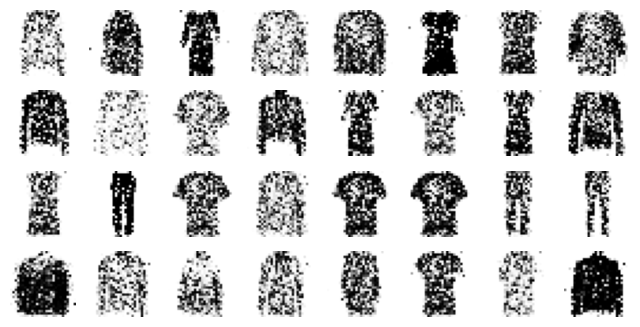
\includegraphics[width=0.85\textwidth]{figures/GAN生成图.png}
    \caption{GAN生成图}
    \label{GAN生成图}
\end{figure}

\subsection{自然语言处理}

\subsubsection{循环神经网络}
循环神经网络(RNN)把神经网络在时序预测上的能力大大推进了,循环神经网络上一个神经元的输出会和新的输入一起进入下一个神经元,从而有了短期记忆的能力,刚开始输入的特征的一部分会进入下一个神经元,但往后,原始特征就逐渐消失了,比如刚开始输入100,后来经过5个神经元计算输出的是-20,并且跟着新的输入一起进入第6个神经元,因此后来改进出了长短期记忆神经网络(LSTM,Long-Short Term Memory)和GRU(Gate Recurrent Unit)模型,这都是RNN的变种,引入了长期记忆机制,从而更好地保留了原始特征,但它们也只是一定程度增加了记忆力。

\subsubsection{注意力机制}
注意力机制(attention)也在大型数据的模型上淘汰了RNN、LSTM和GRU,在注意力机制中引入位置编码概念,使得网络可以保留极长的记忆,基于注意力机制的开山之作Attention Is All You Need\footnote{https://arxiv.org/abs/1706.03762}构建的Transformer模型最初只是用于机器翻译,但是后来也被扩展到了计算机视觉领域。如前面提到的,注意力机制是当今深度学习领域的最流行的前沿技术之一。

\subsection{其他模型}
\subsubsection{自动编码器}
自动编码器的原理很巧妙也很简单,对于一个MLP,我的输入是x,要拟合的对象也是x。这也就是AI歌手的训练方法,声音数据是可以量化的,假如声音数据是x,模型是model,那么训练时就写为\verb|model.fit(x, x)|,模型要拟合输入的数据,使得输出也很接近原来的数据,当我换其他声音数据输入进去,神经网络会调整这个新声音使得输出数据类似x的音色。你可能会担心神经元对原来的x不做任何改变——这样输出也是x,但这几乎不可能,因为每个神经元的参数$w$和$b$是不一样的,激活函数也会调整输出,单个神经元几乎不可能有输入等于输出的情况。

\section{强化学习}

机器学习可分为三大类:监督学习、非监督学习和强化学习,其中有特征有标签训练处理的模型叫监督学习,因为人们会告诉模型输出应该是什么;只有特征没有标签的是无监督学习,比如聚类算法,通过K-mean算法可以把若干散点进行聚类,人们无需事先规定哪些点是同一类。

强化学习,也有称增强学习的。深度学习大多是监督学习,必须有先验的数据进行训练。强化学习通常没有先验的数据(也可能有),想象一个机器人买股票,它可以看到过去一段时间的股票价格,要决定当前是买还是卖,刚开始机器人没有任何经验,它的交易几乎是随机的,但是在多次尝试中,有几次偶然的交易使得机器人获利,大量亏损和获利的案例就可以用来训练机器人,但是训练方法和深度学习是有很大差别的。

上述股票交易机器人,本质上也是一个模型,但是它不做涨跌预测,比如预测下一个k线是涨,然后跟着10个跌停,那实际上这个预测没什么用,模型要给出买入或者卖出的价值,这个价值会连同后续的收益一起计算,这样模型必须学会对后面的行情负责。比如我喂给一个训练好的模型过去100天的k线数据,然后模型可能预测买入的潜在价值是-10,那么不买,即便次日是涨,也不买,果然,后面连续跟着几个大跌,模型就避开了这些损失。然而在深度学习中,模型很难对后续的结果负责,通常只是预测明天是涨是跌,并且以此定交易策略。

在强化学习中也可以引入神经网络,此时称为深度强化学习,但网络在模型中只是一个小零件,强化学习模型本身就类似一台汽车,神经网络模型是汽车的发动机,此外还有大量其他的部件需要手动完成,比如模型的环境问题,股票机器人的环境是股市,但是股市软件是给人看的,程序无法理解,就还需要人为收集数据整理成一个程序能给识别的环境,OpenAI开源了gym环境便于简单练习,但是大部分实际场景的环境是要手动构建的,这也是困难之处。

在具有良好GPU或者TPU的设备上,神经网络的训练是比较快的,强化学习的训练慢是因为和环境交互的慢,即便你有一台好设备。

如果读者对强化学习感兴趣,建议先学完深度学习的各个基本模型,然后可以尝试强化学习。

\chapter{后记}

本小册子实际上是对《机器学习实战-基于Scikit-Learn、Keras和Tensorflow》及其作者Aurélien Géron的拙劣模仿和致敬,在前言和第\ref{route}章中均有提到,《机器学习实战》在笔者学习的过程中给予了重要帮助和指导和很多快乐,笔者真正学到脑子里的也不过它的冰山一角,但是也实在产生了极大的震撼。

本小册子基于笔者在学习机器学习基础之后对MLP的综合理解,也给出了后续研究的介绍,\textbf{如果能给帮助读者理解MLP、产生一些新的思考甚至确定未来的研究方向,本小册子也就达到了目的。}

对本小册子有任何问题或者修改建议,可以通过封面提供的邮件联系我,或者通过其他方式直接联系我。

\end{document}
